\exercisesection{3}

\begin{enumerate}
\def\labelenumi{\arabic{enumi}.}
\tightlist
\item
  \begin{enumerate}
  \def\labelenumii{(\alph{enumii})}
  \tightlist
  \item
    Let A be a ring which is not necessarily commutative and \(I_{s}\) (resp. \(I_{d}\) ) the set of elements of A which have no left (resp. right) inverse. Show that the following conditions are equivalent: (1) the sum of two elements of \(I_{s}\) belongs to \(I_{s}\) ; (2) \(I_{s}\) is a left ideal; (3) there is a greatest left ideal J in the set of left ideals \(\neq A\) . If these conditions hold, the opposite ring \(A^{0}\) also satisfies these conditions, \(I_{s} = I_{d} = J\) , J is the unique maximal (left or right) ideal of A and hence the Jacobson radical of A, every element \(x \notin J\) is invertible and A/J is a field (cf Algebra, Chapter VIII, §6, no. 3). Then we also say that A is a local ring.
  \end{enumerate}
\end{enumerate}

\begin{enumerate}
\def\labelenumi{(\alph{enumi})}
\setcounter{enumi}{1}
\tightlist
\item
  Show that in a local ring there exists no idempotent other than 0 and 1.
\end{enumerate}

\begin{enumerate}
\def\labelenumi{\arabic{enumi}.}
\setcounter{enumi}{1}
\tightlist
\item
  \begin{enumerate}
  \def\labelenumii{(\alph{enumii})}
  \tightlist
  \item
    Let A be a (commutative) local ring whose maximal ideal m is principal and such that \(\bigcap_{n\geqslant1}m^{n}=0\) (cf.~Chapter III, §3, no. 2, Corollary to Proposition 4). Show that the only ideals \(\neq0\) and \(\neq A\) of A are the powers \(m^{n}\) ; deduce that A is Noetherian and is *either a discrete valuation ring (Chapter VI)* or a quasi-principal ring in which 1 is an indecomposable idempotent (Algebra, Chapter VII, §1, Exercise 6).
  \end{enumerate}
\end{enumerate}

\begin{enumerate}
\def\labelenumi{(\alph{enumi})}
\setcounter{enumi}{1}
\tightlist
\item
  Let A be the ring of germs at the point t = 0 of real-valued functions defined and continuous in a neighbourhood of 0 and differentiable at the point 0 (General Topology, Chapter I, 3rd ed., § 6, no. 10). Show that A is a local ring whose maximal ideal m is generated by the germ of the function \(j: t \mapsto t; m^{n} \neq 0\) for all n but A is not a principal ideal domain. If c is the germ of the function \(t \mapsto \exp(-1/t^{2})\) and p a prime ideal of A not containing c, show that the quotient ring B = A/p is a local integral domain which is not a principal ideal domain and in which the maximal ideal is principal.
\end{enumerate}

¶ 3. Let A be a local ring (not necessarily commutative, cf.~Exercise 1) and m its Jacobson radical.

\begin{enumerate}
\def\labelenumi{(\alph{enumi})}
\item
  Let L be a free left A-module and \(x \neq 0\) an element of L. Let \((e_{\iota})_{\iota \in I}\) be a basis of L for which the number of components \(\neq 0\) of x is the least possible; if \(x = \sum_{\iota \in I} \xi_{\iota} e_{\iota}\) , let J be the set of \(\iota \in I\) such that \(\xi_{\iota} \neq 0\) . Show that none of the \(\xi_{\iota} (\iota \in J)\) belongs to the right ideal of A generated by the others.
\item
  With the hypotheses and notation of (a), let P, Q be two complementary submodules of L such that \(x \in P\) ; for all \(\iota \in I\) , let \(e_{\iota} = y_{\iota} + z_{\iota}\) , where \(y_{\iota} \in P\) , \(z_{\iota} \in Q\) . Show that the family of \(y_{\iota}\) for \(\iota \in J\) and \(e_{\iota}\) for \(\iota \notin J\) is a basis of L. (Prove, using (a), that, if \(z_{\kappa} = \sum_{\iota \in I} \zeta_{\kappa_{\iota}} e_{\iota}\) , the components \(\zeta_{\kappa_{\iota}}\) such that \(\kappa \in J\) and \(\iota \in J\) necessarily belong to m and use Corollary 2 to Proposition 4.) Deduce that there exists a free submodule of P which contains x and is a direct factor of P.
\item
  Show that every projective A-module P is free (using Kaplansky's Theorem (Algebra, Chapter II, § 2, Exercise 4), reduce it to the case where P is generated by a countable family of elements and apply (b) to this case).
\item
  Give an example of a local ring A and a flat A-module M which is not free and satisfies mM = M (take \(A = \mathbf{Z}_{(p)}\) ). *(In Chapter III, § 3, we shall give examples of faithfully flat A-modules which are not free over a Noetherian local ring A.)*
\item
  Let A be a local ring and M a finitely generated flat A-module. Show that M is a free A-module (use Exercise 23 (e) of Chapter I, § 2).
\end{enumerate}

\begin{enumerate}
\def\labelenumi{\arabic{enumi}.}
\setcounter{enumi}{3}
\item
  Let A be a local ring (not necessarily commutative) and m its Jacobson radical. Let M and N be two free A-modules (finitely generated or not) and \(u: M \rightarrow N\) a homomorphism such that \(1 \otimes u: M/mM \rightarrow N/mN\) is bijective. Show that u is bijective. (Prove first that u is surjective and then that u is injective, reducing it to the case where M and N are finitely generated and using respectively Corollary 1 to Proposition 4 and Proposition 6.)
\item
  Show by an example that Proposition 7 does not extend to the case where the local ring A is not reduced.
\item
  \begin{enumerate}
  \def\labelenumii{(\alph{enumii})}
  \tightlist
  \item
    Let M be the Z-module defined in Algebra, Chapter VII, §3, Exercise 22 (h); let T be the torsion submodule of M. Show that, for every prime number p, the submodule \(\mathrm{T}_{(p)}\) of \(\mathrm{M}_{(p)}\) is a direct factor of \(\mathrm{M}_{(p)}\) , although T is not a direct factor of M.
  \end{enumerate}
\end{enumerate}

\begin{enumerate}
\def\labelenumi{(\alph{enumi})}
\setcounter{enumi}{1}
\tightlist
\item
  Let \(\mathbf{M}\) be the \(\mathbf{Z}\) -module defined in Algebra, Chapter VII, § 3, Exercise 5; show that, for every prime number \(p\) , \(\mathrm{M}_{(p)}\) is a free \(\mathbf{Z}_{(p)}\) -module, although \(\mathbf{M}\) is not a free \(\mathbf{Z}\) -module.
\end{enumerate}

\begin{enumerate}
\def\labelenumi{\arabic{enumi}.}
\setcounter{enumi}{6}
\item
  Let A be a ring and \((\mathrm{S}_{\lambda})_{\lambda \in L}\) a family of multiplicative subsets of A such that, for every maximal ideal m of A, there exists \(\lambda \in L\) such that \(m \cap S_{\lambda} = \varnothing\) (cf.~§2, Exercise 8). Let M, N be two A-modules and u: M → N a homomorphism. For u to be surjective (resp. injective, bijective, zero), it is necessary and sufficient that, for all \(\lambda \in L\) , \(S_{\lambda}^{-1}u\) : \(S_{\lambda}^{-1}M \to S_{\lambda}^{-1}N\) be so. How can the Corollaries to Theorem 1 of no. 3 be generalized?
\item
  Let A be a ring, B an A-algebra (not necessarily commutative) and E a finitely generated left B-module.
\end{enumerate}

\begin{enumerate}
\def\labelenumi{(\alph{enumi})}
\item
  Let S be a multiplicative subset of A and let \(S^{-1}B = S^{-1}A \otimes_{A} B\) be given its \(S^{-1}A\) -algebra structure; \(S^{-1}E\) can then be considered as a left \(S^{-1}B\) -module (Algebra, Chapter VIII, § 7, no. 1) isomorphic to \(S^{-1}B \otimes_{B} E\) . Show that, if E is a flat B-module, \(S^{-1}E\) is a flat \(S^{-1}B\) -module.
\item
  Let \((\mathbf{S}_{\lambda})_{\lambda \in L}\) be a family of multiplicative subsets of A such that, for every maximal ideal m of A, there exists \(\lambda \in L\) such that \(m \cap S_{\lambda} = \varnothing\) . Show that \(\bigoplus_{\lambda \in L} S_{\lambda}^{-1} B\) is a faithfully flat B-module (left or right; cf.~§ 2, Exercise 8). Show that, if, for all \(\lambda \in L\) , \(S_{\lambda}^{-1} E\) is a flat (resp. faithfully flat) \(S_{\lambda}^{-1} B\) -module, then E is a flat (resp. faithfully flat) B-module (use Chapter I, § 3, Exercise 9, with \(C_{\lambda} = S_{\lambda}^{-1} A\) ).
\item
  Suppose that the \(S_{\lambda}\) satisfy condition (b) and that L is finite. Show that, if, for every \(\lambda \in L\) , \(S_{\lambda}^{-1}E\) is a finitely generated projective \(S_{\lambda}^{-1}B\) -module, then E is a finitely generated projective B-module.
\end{enumerate}

\begin{enumerate}
\def\labelenumi{\arabic{enumi}.}
\setcounter{enumi}{8}
\item
  Show that, for a (commutative) ring A to be absolutely flat (Chapter I, § 2, Exercise 17), it is necessary and sufficient that, for every maximal ideal m of A, \(A_{m}\) be a field (note that an absolutely flat local ring is necessarily a field and use the Corollary to Proposition 15).
\item
  Let A, B be two rings, \(\rho: A \rightarrow B\) a homomorphism, q a prime ideal of B and \(p = \bar{\rho}^{-1}(q)\) . Suppose that there exists a B-module N such that \(N_{q}\) is a flat A-module which is not reduced to 0 and \(N_{q}\) is a finitely generated \(A_{p}\) -module; then the prime ideal p is minimal in A. (Observe that \(N_{p}\) is then a faithfully flat \(A_{p}\) -module and use Corollary 4 to Proposition 11 of §2, no. 5.)
\item
  Let A be a ring, a an ideal of A and S the multiplicative subset of A consisting of the elements whose canonical images in A/a are not divisors of 0; let \(\Phi\) be the set of maximal elements of the set of ideals of A not meeting S (such that the ideals \(p \in \Phi\) are prime, cf.~§2, no. 5, Proposition 11). Show that a is the intersection of its saturations with respect to the ideals \(p \in \Phi\) (reduce it to the case where a = 0 and use Corollary 1 to Theorem 1).
\end{enumerate}

¶ 12. Let \(A = \prod_{i=1}^{n} A_i\) be the product of a finite family of local rings \(A_i\) , canonically identified with ideals of \(A\) . Let \(B\) be a subring of \(A\) such that \(\text{pr}_i B = A_i\) for \(1 \leqslant i \leqslant n\) . Show that \(B\) is the direct composition of at most \(n\) local rings and can only be the direct composition of \(n\) local rings if \(B = A\) . (Proceed by induction on \(n\) , considering the ideals \(a_i = B \cap A_i\) of \(B\) . Examine successively the case where \(a_i = A_i\) for at least one index \(i\) and the case where \(a_i \neq A_i\) for all \(i\) . Note that, if \(a_i \neq A_i\) , every maximal ideal of \(B\) contains \(a_i\) , and considering the ring \(B / a_i\) , conclude that there are at most \(n - 1\) distinct maximal ideals in \(B\) ; if then \(B\) is not a local ring, reduce it to the case where \(a_j = A_j\) for some \(j \neq i\) using the induction hypothesis and Exercise 1 (b).) Give an example where \(n > 1\) and \(B\) is a local ring but not isomorphic to any \(A_t\) (take the \(A_t\) to be algebras over the same field \(K\) , whose maximal ideals \(m_t\) are of zero square).

¶ 13. Let G be a finite group whose order n is a power \(p^{f}\) of a prime number p and K a field of characteristic p.

\begin{enumerate}
\def\labelenumi{(\alph{enumi})}
\item
  Let E be a finite set on which G operates (Algebra, Chapter I, § 7, no. 2); if \(E'\) is the set of elements of E which are invariant for all \(g \in G\) , show that \(\text{Card}(E) \equiv \text{Card}(E') \pmod{p}\) . Deduce that, if G is not reduced to its identity element e, the centre Z of G is not reduced to e (make G operate on itself by inner automorphisms). Conclude that G is solvable (Algebra, Chapter I, § 6, Exercise 14).
\item
  Let V be a vector space over K and \(\rho\) a homomorphism of G to \(\mathbf{GL}(V)\) . Let \(V'\) be the set of \(x \in V\) which are invariant under the linear mappings \(\rho(g)\) , where \(g \in G\) . Show that, if \(V'\) is reduced to 0, V is necessarily reduced to 0. (If \(x \in V\) and \(x \neq 0\) , apply (a) to the additive subgroup E of V generated by the elements \(\rho(g).x\) , where \(g \in G\) .)
\item
  Let \(\mathbf{A} = \mathbf{K}^{(\mathbf{G})}\) be the algebra of the group \(\mathbf{G}\) over \(\mathbf{K}\) (Algebra, Chapter III, § 1) and let \(\mathbf{I}\) be the vector subspace of \(\mathbf{A}\) (over \(\mathbf{K}\) ) generated by the elements \(1 - g\) where \(g \in \mathbf{G}\) . Show that \(\mathbf{I}\) is the Jacobson radical of \(\mathbf{A}\) and that \(\mathbf{A} / \mathbf{I}\) is isomorphic to \(\mathbf{K}\) (use (b) and the definition of Jacobson radical); deduce that \(\mathbf{I}\) is nilpotent.
\item
  Let V be a finitely generated A-module and V' the set of elements x of V such that g.x = x for all \(g \in G\) . Show that the following inequalities hold
\end{enumerate}

\[
(*) \dim_ {\mathbb {K}} (\mathrm{V}) \leqslant n. \dim_ {\mathbb {K}} (\mathrm{V} / \mathrm{IV}); \quad (* *) \dim_ {\mathbb {K}} (\mathrm{V}) \leqslant n. \dim_ {\mathbb {K}} (\mathrm{V} ^ {\prime}).
\]

(To establish (*), use Corollary 2 to Proposition 4; deduce (**) by considering the dual of the vector space V over K.) For the two sides of the inequality (*) (resp. (**)) to be equal, it is necessary and sufficient that V be a free A-module (cf.~Corollary 1 to Proposition 5).

\begin{enumerate}
\def\labelenumi{\arabic{enumi}.}
\setcounter{enumi}{13}
\tightlist
\item
  Let A be a ring, which is not necessarily commutative and whose Jacobson radical m is such that A/m is a field, and M a finitely generated free A-module.
\end{enumerate}

\begin{enumerate}
\def\labelenumi{(\alph{enumi})}
\item
  Let \(\mathbf{M}'\) be another finitely generated free A-module and \(u: \mathbf{M} \to \mathbf{M}'\) a homomorphism such that \(u(\mathbf{M})\) is a direct factor of \(\mathbf{M}'\) ; the number \(\dim(\mathbf{M})\) is called the rank of \(u\) and denoted by \(\operatorname{rg}(u)\) . For such a homomorphism \(\operatorname{Ker}(u)\) is a direct factor of \(\mathbf{M}\) and \(\operatorname{rg}(u) = \dim(\mathbf{M}) - \dim(\operatorname{Ker}(u))\) ; for \(u\) to be injective (resp. surjective), it is necessary and sufficient that \(\operatorname{rg}(u) = \dim(\mathbf{M})\) (resp. \(\operatorname{rg}(u) = \dim(\mathbf{M}')\) ). The transpose \(^t u\) is such that \(^t u(\mathbf{M}'*)\) is a direct factor of \(\mathbf{M}^*\) and \(\operatorname{rg}(^t u) = \operatorname{rg}(u)\) .
\item
  Let \(n = \dim(\mathbf{M})\) . The direct factors of \(\mathbf{M}\) of dimension 1 (resp. \(n - 1\) ) are called lines (resp. hyperplanes). An automorphism \(u \in \mathbf{GL}(\mathbf{M})\) distinct from the identity is called a transvection if there exists a hyperplane \(\mathbf{H}\) of \(\mathbf{M}\) all of whose elements are invariant under \(u\) ; then \(u(x) = x + a\phi(x)\) , where \(\phi\) is a linear form on \(\mathbf{M}\) such that \(\mathbf{H} = \operatorname{Ker}(\phi)\) and \(a \in \mathbf{H}\) ; obtain the converse. If \(\mathbf{A}\) is commutative, show that every automorphism \(u \in \mathbf{GL}(\mathbf{M})\) of determinant 1 is a product of transvections (observe that, in the matrix of \(u\) with respect to any basis of \(\mathbf{M}\) , every column contains at least one invertible element of \(\mathbf{A}\) and a matrix of the form \(I + E_{ij} (i \neq j)\) is the matrix of a transvection).
\item
  Give an example of an automorphism \(u \in \mathbf{GL}(\mathbf{M})\) such that the kernel of \(1 - u\) is not a direct factor of \(\mathbf{M}\) (take \(\mathbf{A}\) to be the local ring \(\mathbf{K}[[\mathbf{X}]]\) of formal power series in one indeterminate over a field \(\mathbf{K}\) and \(\mathbf{M} = \mathbf{A}\) ).
\item
  Give an example of direct factors N, P of M (necessarily free) such that \(N + P\) and \(N \cap P\) are not direct factors of M. (Take A = K{[}X{]}/(X²), where K is a field and M = A².)
\end{enumerate}

¶ 15. Let A be a (commutative) ring and M an A-module.

\begin{enumerate}
\def\labelenumi{(\alph{enumi})}
\item
  For a submodule \(M'\) of M to be pure (Chapter I, §2, Exercise 24), it is necessary and sufficient that, for every maximal ideal m of A, \(M_{m}'\) be a pure sub- \(A_{m}\) -module of \(M_{m}\) (use Theorem 1 of no. 3).
\item
  Suppose that A is a local ring with maximal ideal m and M a finitely generated free A-module. For a finitely generated submodule \(M'\) of M to be pure, it is necessary and sufficient that it be a direct factor of M. (Using Corollary 1 to Proposition 5 of no. 2, reduce it to proving that, if \(M' \subset mM\) , \(M'\) can only be a pure submodule of M if \(M' = 0\) .)
\end{enumerate}

\begin{enumerate}
\def\labelenumi{\arabic{enumi}.}
\setcounter{enumi}{15}
\tightlist
\item
  Let \((\mathbf{A}_{\lambda}, f_{\mu \lambda})\) be a direct system of local rings, such that the \(f_{\mu \lambda}\) are local homomorphisms; let \(m_{\lambda}\) be the maximal ideal of \(\mathbf{A}_{\lambda}\) and \(\mathbf{K}_{\lambda} = \mathbf{A}_{\lambda} / m_{\lambda}\) . Then \(\mathbf{A} = \varinjlim \mathbf{A}_{\lambda}\) is a local ring whose maximal ideal is \(m = \varinjlim m_{\lambda}\) and residue field is \(\mathbf{K} = \varinjlim \mathbf{K}_{\lambda}\) . Moreover, if \(m_{\mu} = \mathbf{A}_{\mu} m_{\lambda}\) for \(\lambda < \mu\) , then \(m = Am_{\lambda}\) for all \(\lambda\) .
\end{enumerate}

\exercisesection{4}

\begin{enumerate}
\def\labelenumi{\arabic{enumi}.}
\item
  Let \((\mathbf{X}_{\alpha}, f_{\alpha\beta})\) be an inverse system of topological spaces, whose indexing set is directed, \(X = \varprojlim X_{\alpha}\) and \(f_{\alpha}\) be the canonical mapping from X to \(X_{\alpha}\) . Suppose that, for all \(\alpha, f_{\alpha}\) is surjective; show that, if the \(X_{\alpha}\) are irreducible, X is irreducible (cf.~General Topology, Chapter I, §4, no. 4, Corollary to Proposition 9). In particular, every product of irreducible spaces is irreducible.
\item
  A point \(x\) in an irreducible space \(\mathbf{X}\) is called generic if \(\{x\}\) is everywhere dense in \(\mathbf{X}\) .
\end{enumerate}

\begin{enumerate}
\def\labelenumi{(\alph{enumi})}
\tightlist
\item
  If \(\mathbf{X}\) is a Kolmogoroff space (General Topology, Chapter I, § 1, Exercise 2), it admits at least one generic point; if \(\mathbf{X}\) is an accessible space (General
\end{enumerate}

Topology, Chapter I, § 8, Exercise 1), it cannot admit a generic point unless it consists of a single point.

\begin{enumerate}
\def\labelenumi{(\alph{enumi})}
\setcounter{enumi}{1}
\item
  Give an example of an infinite irreducible accessible space (cf.~General Topology, Chapter I, § 8, Exercise 5).
\item
  Let X, Y be two irreducible spaces each admitting a generic point; suppose also that Y admits only one generic point y. Let \(f: X \to Y\) be a continuous mapping; for \(f(X)\) to be dense in Y, it is necessary and sufficient that, for every generic point x of X, \(f(x) = y\) .
\item
  Let \((\mathbf{X}_{\alpha}, f_{\alpha \beta})\) be an inverse system of irreducible spaces whose indexing set is directed; suppose that each of the \(\mathbf{X}_{\alpha}\) admits a single generic point \(x_{\alpha}\) . Show that, if, for \(\alpha \leqslant \beta, f_{\alpha \beta}(\mathbf{X}_{\beta})\) is dense in \(\mathbf{X}_{\alpha}\) , then \(\mathbf{X} = \varprojlim \mathbf{X}_{\alpha}\) is irreducible and admits a single generic point (same method as in Exercise 1).
\end{enumerate}

\begin{enumerate}
\def\labelenumi{\arabic{enumi}.}
\setcounter{enumi}{2}
\item
  Let X be a topological space and \((Y_{\alpha})\) a right directed family of subspaces of X; show that if each of the subspaces \(Y_{\alpha}\) is irreducible and X is the union of the family \((Y_{\alpha})\) , X is irreducible. Deduce an example where X is a Kolmogoroff space, each of the \(Y_{\alpha}\) admits a generic point, but X does not admit a generic point.
\item
  Let Y be an irreducible space admitting a single generic point y, X a topological space and \(f: X \rightarrow Y\) a continuous mapping.
\end{enumerate}

\begin{enumerate}
\def\labelenumi{(\alph{enumi})}
\item
  For every irreducible component \(\mathbf{Z}\) of \(\mathbf{X}\) meeting \(f^{-1}(y), f(\mathbf{Z})\) is dense in \(\mathbf{Y}\) .
\item
  Give an example where \(f(\mathbf{X})\) is dense in \(\mathbf{Y}\) but \(f^{-1}(y)\) is empty (take \(\mathbf{X}\) to be a subspace of \(\mathbf{Y}\) ).
\item
  Show that, if \(\mathbf{Z}\) admits a generic point \(z\) and \(f(\mathbf{Z})\) is dense in \(\mathbf{Y}\) , then \(f(z) = y\) and \(z\) is a generic point of \(\mathbf{Z} \cap f^{-1}(y)\) .
\end{enumerate}

\begin{enumerate}
\def\labelenumi{\arabic{enumi}.}
\setcounter{enumi}{4}
\item
  Let G be a connected semi-topological group (General Topology, Chapter III, § 1, Exercise 2). Show that, if G only admits a finite number of irreducible components, it is necessarily irreducible (observe that the irreducible components are derived from the irreducible component containing the identity element e by left or right translation).
\item
  Let \(\mathbf{X}\) be a topological space.
\end{enumerate}

\begin{enumerate}
\def\labelenumi{(\alph{enumi})}
\item
  Let x be a point of X and U an open neighbourhood of x with only a finite number of irreducible components. Show that there exists a neighbourhood V of x such that every neighbourhood contained in V is connected.
\item
  Suppose that every point of X possesses an open neighbourhood with only a finite number of irreducible components. Show that the following properties are equivalent:
\end{enumerate}

(α) The irreducible components of X are open.

(β) The irreducible components of X are identical with its connected components.

(γ) The connected components of X are irreducible.

(δ) Two distinct irreducible components of X do not meet.

\begin{enumerate}
\def\labelenumi{\arabic{enumi}.}
\setcounter{enumi}{6}
\item
  Let X be a compact metrizable space and R an open equivalence relation on X such that the quotient space X/R is irreducible. Show that there exists a point \(x \in X\) whose class mod. R is everywhere dense. (Note first that every open subset of X which is saturated with respect to R is everywhere dense. Then use Baire's Theorem.)
\item
  Show that the product of two Noetherian spaces is Noetherian. (If X and Y are Noetherian spaces and A is an open subset of \(X \times Y\) , show that, for all \(x \in pr_{1}A\) , there exists an open neighbourhood V of x such that \(V \times A(x) \subset A\) and deduce that A is quasi-compact.)
\item
  \begin{enumerate}
  \def\labelenumii{(\alph{enumii})}
  \tightlist
  \item
    Show that the prime spectrum of a commutative ring is a Kolmogoroff space (General Topology, Chapter I, § 1, Exercise 2), in which every irreducible component admits a (unique) generic point.
  \end{enumerate}
\end{enumerate}

\begin{enumerate}
\def\labelenumi{(\alph{enumi})}
\setcounter{enumi}{1}
\tightlist
\item
  Let A be an integral domain and \(\xi = (0)\) the generic point of \(\mathbf{X} = \operatorname{Spec}(\mathbf{A})\) . For the point \(\xi\) to be isolated in X, it is necessary and sufficient that the intersection of the prime ideals \(\neq 0\) of A be an ideal \(\neq 0\) . Give an example of a local ring with this property.
\end{enumerate}

\begin{enumerate}
\def\labelenumi{\arabic{enumi}.}
\setcounter{enumi}{9}
\item
  Let A be a ring and N its nilradical. For the spectrum of A to be discrete, it is necessary and sufficient that A/N be the direct composition of a finite number of fields.
\item
  Let K be a field, A the polynomial ring K{[}X, Y{]} and B the quotient ring A/(XY); show that Spec(B) is connected but has two distinct irreducible components.
\item
  Let Y be a completely regular space, \(\mathbf{A} = \mathcal{C}^{\infty}(\mathbf{Y}; \mathbf{R})\) and \(\mathbf{B} = \mathcal{C}(\mathbf{Y}; \mathbf{R})\) . Show that the Stone-Čech compactification \(\beta Y\) of Y is canonically identified with an everywhere dense subspace of \(\operatorname{Spec}(A)\) and with an everywhere dense subspace of \(\operatorname{Spec}(B)\) .
\item
  Let \(\mathbf{A}\) be a ring and \(\mathbf{X} = \operatorname{Spec}(\mathbf{A})\) its spectrum.
\end{enumerate}

\begin{enumerate}
\def\labelenumi{(\alph{enumi})}
\item
  If a subset F of X is closed, it has the following two properties: (α) for all p ∈ F, V(p) ⊂ F; (β) for all p ∉ F, there exists a closed subset of V(p) which contains F ∩ V(p) and does not contain p.
\item
  Suppose X is Noetherian. Show that every subset F of X with properties \((\alpha)\) and \((\beta)\) of (a) is closed in X (consider the irreducible components of \(\overline{F}\) and use Exercise 9 (a)).
\item
  With the notation of Exercise 12, take Y to be the interval {[}0, 1{]} of R. Show that Y is not closed in X = Spec(A) (cf.~§ 2, Exercise 15) but satisfies conditions ( \(\alpha\) ) and ( \(\beta\) ) of (a).
\end{enumerate}

\begin{enumerate}
\def\labelenumi{\arabic{enumi}.}
\setcounter{enumi}{13}
\tightlist
\item
  Let A be a ring, \(\mathbf{X} = \operatorname{Spec}(\mathbf{A})\) its spectrum and P the set of minimal prime ideals of A.
\end{enumerate}

\begin{enumerate}
\def\labelenumi{(\alph{enumi})}
\item
  Let \(R_{\mathfrak{p},\mathfrak{p}^{\prime}}\) be the symmetric and reflexive relation: ``there exists a prime ideal \(\mathfrak{p}''\) of A containing \(\mathfrak{p} + \mathfrak{p}'''\) between the elements \(\mathfrak{p},\mathfrak{p}'\) of P; let S be the equivalence relation whose graph is the smallest of the graphs of equivalences containing the graph of R (Set Theory, Chapter II, § 6, Exercise 10). Show that, if I is an equivalence class with respect to S, the set \(V_{I} = \bigcup_{\mathfrak{p}\in I}V(\mathfrak{p})\) is connected.
\item
  Show that, if P is finite (and in particular if A is Noetherian), the \(V_{I}\) are the connected components of X. Does this result extend to the case where P is infinite (cf.~Exercise 12)?
\end{enumerate}

¶ 15. Let A be a ring and a a finitely generated ideal of A. Show that the following properties are equivalent: (α) \(a^{2} = a\) ; (β) A is generated by an idempotent; (γ) V(a) is both open and closed in X = Spec(A) and a is minimal among the ideals b such that r(b) = r(a) (use § 2, Corollary 3 to Proposition 4). Give an example where \(a^{2} = a\) , a is not finitely generated and does not contain an idempotent (cf.~§ 2, Exercise 15).

¶ 16. (a) Let A be an absolutely flat (commutative) ring (Chapter I, §2, Exercise 17). Show that X = Spec(A) is a totally disconnected compact space, that every prime ideal p of A is maximal and that \(A_{p}\) is canonically isomorphic to the field A/p (show first that, for all f ∈ A, V(f) is both open and closed in X; on the other hand use §3, Exercise 9).

\begin{enumerate}
\def\labelenumi{(\alph{enumi})}
\setcounter{enumi}{1}
\tightlist
\item
  Show that the mapping \(\mathfrak{a}\mapsto\mathrm{V}(\mathfrak{a})\) is a bijection of the set of ideals of A onto the set of closed subsets of X. Moreover, the following conditions are equivalent: ( \(\alpha\) ) V(a) is open; ( \(\beta\) ) a is finitely generated; ( \(\gamma\) ) a is generated by an idempotent; ( \(\delta\) ) A/a is a projective A-module.
\end{enumerate}

* (c) Let \(\tilde{A}\) be the structure sheaf of rings over \(X\) . Show that every \(\tilde{A}\) -Module \(\mathcal{F}\) is of the form \(\tilde{E}\) , where \(E\) is an A-module defined up to a unique isomorphism (take \(E = \Gamma(X, \mathcal{F})\) and use the fact that every point of \(X\) admits a fundamental system of neighbourhoods which are both open and closed). For every ideal \(a\) of \(A\) , show that \(\operatorname{Hom}_A(a, E)\) is identified with \(\Gamma(X - V(a), \tilde{E})\) (note that \(X - V(a)\) is the union of the \(X_e\) , where \(e\) runs through the set of idempotents \(e \in a\) ). Deduce that, for \(E\) to be an injective A-module, it is necessary and sufficient that \(\tilde{E}\) be flabby. *

\begin{enumerate}
\def\labelenumi{(\alph{enumi})}
\setcounter{enumi}{3}
\tightlist
\item
  Let A be a ring and \(\mathfrak{N}\) its nilradical. The following properties are equivalent:
\end{enumerate}

(α) \(A/\mathfrak{N}\) is absolutely flat.

(β) \(\mathbf{X} = \operatorname{Spec}(\mathbf{A})\) is Hausdorff.

(γ) Every point of X is closed (in other words, every prime ideal of A is maximal).

(Use Exercises 9 of § 3.)

¶ 17. * (a) Let X be a totally disconnected compact space and O a sheaf of rings over X such that, for all \(x \in X\) , \(\mathcal{O}_x\) is a commutative field. Show that, if A = \(\Gamma(X, \mathcal{O})\) , the ring A is absolutely flat and its spectrum (with the sheaf of rings \(\tilde{A}\) ) is canonically identified with X (with the sheaf O). (Observe that for all \(f \in A\) the set of \(x \in X\) such that \(f_x = 0\) is both open and closed in X and deduce the existence of \(g \in A\) such that \(f = gf^2\) .) *

\begin{enumerate}
\def\labelenumi{(\alph{enumi})}
\setcounter{enumi}{1}
\item
  Let X be a totally disconnected compact space, K a (commutative) field and A the ring of locally constant mappings from X to K. Show that A is absolutely flat (argue directly or use (a)).
\item
  Let A be the ring of real-valued step functions defined on I = {[}0, 1{[}, whose points of discontinuity are of the form \(k/2^n\) ( \(n \in \mathbf{N}, 0 \leqslant k < 2^n\) ) and which are right continuous. Let \(\mathfrak{S}\) be the set of finite unions of half-open intervals \([x, y[ \subset I\) whose extremities are of the form \(k/2^n\) . For every \(f \in A\) ,
\end{enumerate}

the set \(Z(f) = f^{-1}(0)\) belongs to \(\mathfrak{S}\). If a is an ideal of A, the set \(\mathfrak{B}\) of \(Z(f)\) , where f runs through a, is such that: (1) the intersection of two sets of \(\mathfrak{B}\) belongs to \(\mathfrak{B}\); (2) every set of \(\mathfrak{S}\) containing a set of \(\mathfrak{B}\) belongs to \(\mathfrak{B}\). Obtain the converse. For a to be prime, it is necessary and sufficient that \(\mathfrak{B}\) be the base of a filter which converges to a point of {[}0, 1{]}. Show that A is an absolutely flat reduced ring and that, for every maximal ideal m of A, \(A_{m}\) is isomorphic to the field R. Describe the space Spec(A).

¶ 18. (a) Let Y be a completely regular space. Show that the following conditions are equivalent:

\((\alpha)\) Every prime ideal of \(\mathcal{C}(\mathbf{Y};\mathbf{R})\) is maximal.

(β) Every countable intersection of open subsets of Y is open.

(γ) Every continuous real-valued function on Y is locally constant.

(δ) The ring \(\mathcal{C}(\mathbf{Y};\mathbf{R})\) is absolutely flat.

(Use Exercise 15 (f) of § 2.)

If these hold, the space \(\mathbf{X} = \operatorname{Spec}(\mathcal{C}(\mathbf{Y};\mathbf{R}))\) is canonically identified with the Stone-Čech compactification \(\beta \mathbf{Y}\) of \(\mathbf{Y}\) . Such a space \(\mathbf{Y}\) is called flat.

\begin{enumerate}
\def\labelenumi{(\alph{enumi})}
\setcounter{enumi}{1}
\item
  Every subspace of a flat space is flat. Every completely regular quotient space of a flat space is flat. Every finite product of flat spaces is flat. Every sum of flat spaces is a flat space.
\item
  In a flat space, every countable subspace is closed and discrete. In particular every countable flat space is discrete.
\item
  Every Weierstrassian completely regular space (General Topology, Chapter IX, § 1, Exercise 22) (and a fortiori every compact space), which is flat, is finite.
\item
  The space associated with a non-trivial ultrafilter is extremely disconnected (General Topology, Chapter I, § 11, Exercise 21) but is not flat.
\item
  The discrete space \(\mathbf{N}\) is flat but its Stone-Čech compactification is not flat and the spectra of the rings \(\mathcal{C}(\mathbf{N};\mathbf{R})\) and \(\mathcal{C}^{\infty}(\mathbf{N};\mathbf{R})\) are therefore not isomorphic.
\end{enumerate}

\begin{enumerate}
\def\labelenumi{\arabic{enumi}.}
\setcounter{enumi}{18}
\tightlist
\item
  \begin{enumerate}
  \def\labelenumii{(\alph{enumii})}
  \tightlist
  \item
    Let \(\phi: A \to B\) be a ring homomorphism. Show that, for every ideal \(\mathfrak{b}\) of \(B\) , \(\overline{^a\phi(V(b))} = V(\overline{\phi}^{-1}(b))\) .
  \end{enumerate}
\end{enumerate}

\begin{enumerate}
\def\labelenumi{(\alph{enumi})}
\setcounter{enumi}{1}
\item
  Deduce from (a) that, for \(^{a}\phi(\text{Spec}(B))\) to be dense in \(\text{Spec}(A)\) , it is necessary and sufficient that \(\text{Ker}(\phi)\) be a nil ideal of A.
\item
  Show that, if every \(b \in \mathbf{B}\) may be written as \(b = h\phi(a)\) , where \(h\) is invertible in \(\mathbf{B}\) and \(a \in \mathbf{A}\) , \(^a\phi\) is a homeomorphism of \(\operatorname{Spec}(\mathbf{B})\) onto a subspace of \(\operatorname{Spec}(\mathbf{A})\) .
\end{enumerate}

\begin{enumerate}
\def\labelenumi{\arabic{enumi}.}
\setcounter{enumi}{19}
\item
  Give an example of a ring homomorphism \(\phi: A \to B\) such that every maximal ideal of \(A\) is of the form \(\bar{\phi}(m)\) , where \(m\) is a maximal ideal of \(B\) , but there exist prime ideals of \(A\) which are not inverse images under \(\phi\) of ideals of \(B\) (take \(B\) to be a field).
\item
  Let \((\mathbf{A}_{\alpha}, \phi_{\beta \alpha})\) be a direct system of rings whose indexing set is directed, \(\mathbf{A} = \varinjlim \mathbf{A}_{\alpha}\) and \(\phi_{\alpha}: \mathbf{A}_{\alpha} \to \mathbf{A}\) the canonical homomorphism. If we write \(\mathbf{X}_{\alpha} = \operatorname{Spec}(\mathbf{A}_{\alpha})\) , \((\mathbf{X}_{\alpha}, {}^{a}\phi_{\beta \alpha})\) is an inverse system of topological spaces and, if \(\mathbf{X} = \operatorname{Spec}(\mathbf{A})\) , the \({}^{a}\phi_{\alpha}: \mathbf{X} \to \mathbf{X}_{\alpha}\) form an inverse system of continuous mappings. Show that \(u = \varprojlim {}^{a}\phi_{\alpha}\) is a homeomorphism of \(\mathbf{X}\) onto \(\varprojlim {}^{\infty}\mathbf{X}_{\alpha}\) . (Prove
\end{enumerate}

first that, if, for all \(\alpha\) , \(p_{\alpha}\) is a prime ideal of \(\mathbf{A}_{\alpha}\) such that \(p_{\alpha} = \phi_{\beta \alpha}^{-1}(p_{\beta})\) for all \(\alpha \leqslant \beta\) , the union \(p\) of the \(\phi_{\alpha}(p_{\alpha})\) is a prime ideal of \(\mathbf{A}\) ; conversely, every prime ideal \(p\) of \(\mathbf{A}\) is the union of the \(\phi_{\alpha}(p_{\alpha})\) , where \(p_{\alpha} = \overline{\phi}_{\alpha}(p)\) . Finally, if \(f_{\alpha} \in \mathbf{A}_{\alpha}\) and \(f = \phi_{\alpha}(f_{\alpha})\) , note that the relation \(p \in \mathbf{X}_f\) is equivalent to

\[
u (\mathfrak {p}) \in \overline {{\operatorname{pr}}} _ {\alpha} ^ {- 1} ((\mathrm{X} _ {\alpha}) _ {f _ {\alpha}}).
\]

\begin{enumerate}
\def\labelenumi{\arabic{enumi}.}
\setcounter{enumi}{21}
\tightlist
\item
  \begin{enumerate}
  \def\labelenumii{(\alph{enumii})}
  \tightlist
  \item
    Let M be an A-module and \((\mathbf{N}_{i})\) a finite family of submodules of M. Show that \(\operatorname{Supp}\left(\mathbf{M}/\bigcap_{i}\mathbf{N}_{i}\right)=\bigcup_{i}\operatorname{Supp}(\mathbf{M}/\mathbf{N}_{i})\) (note that \(M/\bigcap_{i}N_{i}\) is isomorphic to a submodule of the direct sum of the \(M/N_{i}\) ).
  \end{enumerate}
\end{enumerate}

\begin{enumerate}
\def\labelenumi{(\alph{enumi})}
\setcounter{enumi}{1}
\item
  Let \(p\) be a prime number; the support of the \(\mathbf{Z}\) -module \(\mathbf{Z}\) is distinct from the closure of the union of the supports of the \(\mathbf{Z}\) -modules \(\mathbf{Z} / p^k\mathbf{Z}\) ( \(k \in \mathbf{N}\) ).
\item
  Let M be the direct sum of the Z-modules \(Z/p^{k}Z\) ( \(k \in N\) ); show that Supp(M) is closed but distinct from V(a), where a is the annihilator of M.
\item
  Let \(\mathbf{N}\) be the direct sum of the \(\mathbf{Z}\) -modules \(\mathbf{Z} / n\mathbf{Z}\) ( \(n \geqslant 1\) ); show that \(\operatorname{Supp}(\mathbf{N})\) is not closed in \(\operatorname{Spec}(\mathbf{Z})\) .
\item
  Deduce from (c) and (d) an example of an A-module M such that, if a is its annihilator, Supp(M) is not closed and its closure is distinct from V(a).
\item
  Show that the support of the \(\mathbf{Z}\) -module \(\prod_{k=1}^{n} (\mathbf{Z}/p^k\mathbf{Z})\) is distinct from the closure of the union of the supports of the factor modules \(\mathbf{Z}/p^k\mathbf{Z}\) .
\end{enumerate}

\begin{enumerate}
\def\labelenumi{\arabic{enumi}.}
\setcounter{enumi}{22}
\item
  Let \(p\) be a prime number; give an example of \(\mathbf{Z}\) -modules \(M, N\) , where \(N\) is finitely generated, such that \(\mathbf{M}_{(p)} \neq 0\) and \(\mathbf{N}_{(p)} \neq 0\) , but \((\mathbf{M} \otimes_{\mathbf{Z}} \mathbf{N})_{(p)} = 0\) (take \(\mathbf{M} = \mathbf{Q}\) ).
\item
  \begin{enumerate}
  \def\labelenumii{(\alph{enumii})}
  \tightlist
  \item
    Let A be a ring and M, N two A-modules such that M is finitely generated. Show that \(\operatorname{Supp}(\operatorname{Hom}_{\mathbf{A}}(\mathbf{M}, \mathbf{N}))\) is contained in the intersection \(\operatorname{Supp}(\mathbf{M}) \cap \operatorname{Supp}(\mathbf{N})\) .
  \end{enumerate}
\end{enumerate}

\begin{enumerate}
\def\labelenumi{(\alph{enumi})}
\setcounter{enumi}{1}
\item
  Give an example where M and N are both finitely presented and \(\operatorname{Supp}(\operatorname{Hom}_{\mathbf{A}}(\mathbf{M},\mathbf{N}))\) is strictly contained in \(\operatorname{Supp}(\mathbf{M}) \cap \operatorname{Supp}(\mathbf{N})\) (take \(\mathbf{A} = \mathbf{Z}_{(p)}\) and \(\mathbf{N} = \mathbf{A}\) ).
\item
  Let M be the Z-module the direct sum of the \(Z/p^{k}Z\) (p prime, \(k \in N\) ). Show that \(\text{Supp}(\text{Hom}_{\mathbf{Z}}(\text{M}, \text{M}))\) is not contained in \(\text{Supp}(\text{M})\) .
\end{enumerate}

\begin{enumerate}
\def\labelenumi{\arabic{enumi}.}
\setcounter{enumi}{24}
\tightlist
\item
  Let A be a Noetherian ring, \(X = \text{Spec}(A)\) its spectrum, M a finitely generated A-module and \(Y = \text{Supp}(M)\) . Let \(Y_k (1 \leqslant k \leqslant n)\) be the distinct connected components of Y.
\end{enumerate}

\begin{enumerate}
\def\labelenumi{(\alph{enumi})}
\item
  Show that there exists a unique decomposition of M as a direct sum \(M = M_{1} \oplus M_{2} \oplus \cdots \oplus M_{n}\) such that \(\text{Supp}(M_{k}) = Y_{k}\) for all k.
\item
  If \(\mathfrak{a} = \operatorname{Ann}(\mathbf{M})\) and \(\mathfrak{a}_k = \operatorname{Ann}(\mathbf{M}_k)\) , show that the \(\mathfrak{a}_k\) are relatively prime in pairs and that \(\prod_{k=1}^{n} \mathfrak{a}_k = \mathfrak{a}\) .
\end{enumerate}

(Using Proposition 17 of no. 4, reduce it to the case where \(\mathfrak{a} = 0\) and \(\mathbf{Y} = \mathbf{X}\) and apply Proposition 15 of no. 3.)

\begin{enumerate}
\def\labelenumi{\arabic{enumi}.}
\setcounter{enumi}{25}
\tightlist
\item
  Let \(\phi: \mathbf{A} \to \mathbf{B}\) be a ring homomorphism such that the mapping
\end{enumerate}

\[
^ {a} \phi : \operatorname{Spec} (\mathbf {B}) \rightarrow \operatorname{Spec} (\mathbf {A})
\]

is surjective. Let N be a finitely generated A-module; show that, if \(u: M \to N\) is an A-module homomorphism such that \(u \otimes 1: M_{(B)} \to N_{(B)}\) is surjective, then u is surjective (apply Proposition 19 of no. 4 to Coker(u)).

\begin{enumerate}
\def\labelenumi{\arabic{enumi}.}
\setcounter{enumi}{26}
\item
  Give an example of a local homomorphism \(\rho: \mathbf{A} \to \mathbf{B}\) and an A-module \(\mathbf{M}\) (not finitely generated) such that \(\operatorname{Supp}(\mathbf{M}_{(\mathbf{B})})\) is not equal to \(a\rho^{-1}(\operatorname{Supp}(\mathbf{M}))\) (take \(\mathbf{A} = \mathbf{Z}_{(p)}\) and \(\mathbf{B} = \mathbf{Z}/p\mathbf{Z}\) for some prime number \(p\) ).
\item
  Give an example of a Z-module M such that, for some prime number p such that \((p) \in \text{Supp}(M)\) , there exists no Z-homomorphism \(\neq 0\) from M to Z/pZ.
\end{enumerate}

\exercisesection{5}

\begin{enumerate}
\def\labelenumi{\arabic{enumi}.}
\item
  Define an endomorphism \(u\) of the \(\mathbf{Z}\) -module \(\mathbf{M} = \mathbf{Z}^{(\mathbf{N})}\) such that, for the prime ideal \(p = (0)\) of \(\mathbf{Z}\) , \(u_{p}\) is an automorphism of \(M_p\) but that there exists no \(f \neq 0\) in \(\mathbf{Z}\) such that \(u_f\) is a surjective endomorphism of \(M_f\) .
\item
  Let K be a field and B the ring of polynomials with coefficients in K in an infinite system of indeterminates \(X_{i}\) ( \(i \in N\) ); let b be the ideal of B generated by the products \(\mathbf{X}_i\mathbf{X}_j\) ( \(i \neq j\) ), A the quotient ring B/b, \(\xi_i\) the class of \(\mathbf{X}_i\) mod. b ( \(i \in \mathbb{N}\) ), p the ideal of A generated by the \(\xi_i\) of index \(i \geqslant 1\) , which is prime, and u the canonical mapping A → A/p.~Show that \(u_p: \mathbf{A}_p \to (\mathbf{A}/\mathfrak{p})_p\) is bijective but that there exists no \(f \in \mathbf{A} - \mathfrak{p}\) such that \(u_f\) is bijective.
\item
  Let A be a ring and P a finitely generated projective A-module. Show that A is isomorphic to a finite product of rings \(\prod_{i\in I}A_{i}\) and P is isomorphic to a product \(\prod_{i\in I}P_{i}\) , where \(P_{i}\) is a projective \(A_{i}\) -module of rank \(n_{i}\) , the \(n_{i}\) being distinct (use Theorem 1 and the fact that \(\operatorname{Spec}(A)\) is quasi-compact).
\item
  Let A be a (commutative) ring and B a (not necessarily commutative) ring containing A. Suppose that the left A-module B is projective and finitely generated. Show that A is a direct factor of B. (Reduce it to the case where A is a local ring and use § 3, no. 2, Corollary 1 to Proposition 5.)
\item
  Let A be a reduced ring and M a finitely generated A-module. Suppose that there exists an integer n \textgreater{} 0 such that, for every homomorphism \(\phi\) of A to a field \(K_{\phi}\) , \([M \otimes_{A} K_{\phi}: K_{\phi}] = n\) . Show that M is a projective module of rank n.~(Reduce it to the case where A is a local ring and use §2, no. 2, Proposition 7.)
\end{enumerate}

¶ 6. Let A be an integral domain, K its field of fractions and M an A-module. Show that the following properties are equivalent:

\((\alpha)\) M is a projective A-module such that \([\mathbf{M} \otimes_{\mathbf{A}} \mathbf{K} : \mathbf{K}]\) is finite.

(β) M is finitely generated projective A-module.

\((\gamma)\) M is finitely generated and, for every maximal ideal m of A, the \(\mathbf{A}_{m}\) -module \(\mathbf{M}_{m}\) is free.

(To show that \((\alpha)\) implies \((\beta)\) , use Algebra, Chapter II, § 5, no. 5, Proposition 9. To show that \((\gamma)\) implies \((\alpha)\) , observe first that M is torsion-free and conclude that, for every prime ideal \(p\) of A, \(M_{p}\) is a free \(A_{p}\) -module of constant rank.)

\begin{enumerate}
\def\labelenumi{\arabic{enumi}.}
\setcounter{enumi}{6}
\tightlist
\item
  Let A be an absolutely flat (commutative) ring (cf.~§ 4, Exercise 16) and let X be its spectrum.
\end{enumerate}

\begin{enumerate}
\def\labelenumi{(\alph{enumi})}
\item
  Let F be a closed subset of X and a the corresponding ideal of A (loc. cit.). Show that M = A/a is a monogenous flat A-module such that \(M_{m}\) is a free \(A_{m}\) -module for all \(m \in X\) , but that M is projective only if F is open.
\item
  Let E be the module the direct sum of the A/m, for \(m \in X\) . Show that E is a flat A-module such that \(E_{m}\) is a free \(A_{m}\) -module of rank 1 for all \(m \in X\) ; for E to be a projective A-module, it is necessary and sufficient that X be finite (note that, if A/m is a projective A-module, m is finitely generated).
\end{enumerate}

\begin{enumerate}
\def\labelenumi{\arabic{enumi}.}
\setcounter{enumi}{7}
\tightlist
\item
  Let A be a ring and M a projective A-module of rank n.~Show that there exists a finitely generated (commutative) A-algebra B such that the A-module
\end{enumerate}

B is faithfully flat and \(\mathbf{M}_{(\mathbf{B})} = \mathbf{M} \otimes_{\mathbf{A}} \mathbf{B}\) is a free B-module of rank \(n\) (use Theorem 1 (d) and Proposition 3). Obtain the converse.

¶ 9. (a) Let A be a ring, \((f_i)_{i \in I}\) a finite family of elements of A generating the ideal A and M an A-module. Suppose given in each of the \(A_{f_i}\) -modules \(M_{f_i}\) an element \(z_i\) such that, for \(i \neq j\) , the canonical images of \(z_i\) and \(z_j\) in \(M_{f_i f_j}\) are equal. Show that there exists a unique \(z \in M\) such that, for all \(i\) , the canonical image of \(z\) in \(M_{f_i}\) is equal to \(z_i\) . (Note that, for every integer \(k > 0\) , there exists a family \((g_i)_{i \in I}\) of elements of A such that \(\sum_{i} g_i f_i^k = 1\) .)

\begin{enumerate}
\def\labelenumi{(\alph{enumi})}
\setcounter{enumi}{1}
\item
  Let A be a ring and P a projective A-module of rank 1. Show that the ring \(\operatorname{End}_{\mathbf{A}}(\mathbf{P})\) is canonically isomorphic to A (use Theorem 3).
\item
  Let A be a ring and P a projective A-module of rank n.~For every endomorphism u of P, there corresponds canonically to \(\wedge^{n}u\) , by (b), an element \(\det(u)\) of A, called the determinant of u, such that \(\det(u \circ v) = (\det u)(\det v)\) for two endomorphisms u, v of P. The element \(\chi_{u}(T) = \det(T.1 - u)\) of A{[}T{]} is called the characteristic polynomial of u (cf.~no. 3, Proposition 4); show that \(\chi_{u}\) is a monic polynomial of degree n and that \(\chi_{u}(u) = 0\) (use (a) and §3, no. 3, Theorem 1). Deduce that, for u to be bijective, it is necessary and sufficient
\end{enumerate}

that \(\det(u)\) be invertible in A. If A is an integral domain, \(\chi_u(T) = \prod_{i=1}^{n} (T - \alpha_i)\) the decomposition into the linear factors of \(\chi_u\) in an algebraically closed extension

of the field of fractions of A, and \(\chi_{q(u)}(T) = \prod_{i=1}^{l} (T - q(\alpha_i))\) for every polynomial \(q \in A[T]\) . Generalize similarly Proposition 14 of Algebra, Chapter VII, § 5, no. 6.

\begin{enumerate}
\def\labelenumi{\arabic{enumi}.}
\setcounter{enumi}{9}
\tightlist
\item
  Let A be a ring and \(E(A)\) the set of classes of finitely generated projective A-modules; let G be the Z-module of formal linear combinations of elements of \(E(A)\) and N the submodule of G consisting of the elements \(\xi - \xi' - \xi''\) , where \(\xi, \xi', \xi''\) are the classes of three projective A-modules M, M', M'' such that there exists an exact sequence
\end{enumerate}

\[
0 \rightarrow \mathrm{M} ^ {\prime} \rightarrow \mathrm{M} \rightarrow \mathrm{M} ^ {\prime \prime} \rightarrow 0
\]

(it amounts to the same to say that M is isomorphic to the direct sum \(M' \oplus M''\) by virtue of Algebra, Chapter II, §2, no. 2). Let \(K(A)\) be the quotient Z-module G/N and, for every finitely generated projective A-module, let \(\kappa(M)\) (or \(\kappa_{A}(M)\) ) be its class in \(K(A)\) .

\begin{enumerate}
\def\labelenumi{(\alph{enumi})}
\item
  Show that there exists on \(K(\mathbf{A})\) a unique commutative ring structure whose addition is that the Z-module \(K(\mathbf{A})\) and multiplication is such that \(\kappa(\mathbf{M})\kappa(\mathbf{N}) = \kappa(\mathbf{M} \otimes_{\mathbf{A}} \mathbf{N})\) for two finitely generated projective A-modules M, N; \(\kappa(\mathbf{A})\) is the unit element of \(K(\mathbf{A})\) .
\item
  For every finitely generated projective A-module M and every integer \(p \geqslant 0\) let \(\lambda^p\) denote the element \(\kappa(\bigwedge^p M)\) of \(K(A)\) . Show that
\end{enumerate}

\[
\lambda^ {p} (\mathbf {M} \oplus \mathbf {N}) = \sum_ {r + s = p} \lambda^ {r} (\mathbf {M}). \lambda^ {s} (\mathbf {N}).
\]

Let \(\lambda_{\mathrm{T}}(\mathbf{M})\) denote the element \(\sum_{p=0}^{\infty} \lambda^{p}(\mathbf{M}) \mathrm{T}^{p}\) in the ring \(K(\mathrm{A})[[\mathrm{T}]]\) of formal power series in one indeterminate over the ring \(K(\mathrm{A})\) ; show that

\[
\lambda_ {\mathbf {T}} (\mathbf {M} \oplus \mathbf {N}) = \lambda_ {\mathbf {T}} (\mathbf {M}) \lambda_ {\mathbf {T}} (\mathbf {N});
\]

derive a homomorphism also written \(x \mapsto \lambda_{\mathrm{T}}(x)\) of \(K(\mathrm{A})\) to the multiplicative group of formal power series of \(K(\mathrm{A})[[\mathrm{T}]]\) whose constant term is equal to 1. Let \(\lambda^{p}(x)\) denote the coefficient of \(T^{p}\) in \(\lambda_{\mathrm{T}}(x)\) ; then

\[
\lambda^ {p} (x + y) = \sum_ {r + s = p} \lambda^ {r} (x) \lambda^ {s} (y)
\]

for all \(x, y\) in \(\mathbf{K}(\mathbf{A})\) .

\begin{enumerate}
\def\labelenumi{(\alph{enumi})}
\setcounter{enumi}{2}
\item
  If \(\mathbf{A}\) is a local ring, the ring \(K(\mathbf{A})\) is canonically identified with \(\mathbf{Z}\) and \(\lambda^p(n) = \binom{n}{p}\). Deduce that, if \(\mathbf{A}\) is the direct composition of \(m\) local rings, \(K(\mathbf{A})\) is isomorphic to \(\mathbf{Z}^m\) .
\item
  Let \(\phi: \mathbf{A} \to \mathbf{B}\) be a ring homomorphism. Show that there exists a unique ring homomorphism \(\phi': \mathbf{K}(\mathbf{A}) \to \mathbf{K}(\mathbf{B})\) such that \(\phi'(\kappa_{\mathbf{A}}(\mathbf{M})) = \kappa_{\mathbf{B}}(\mathbf{M}_{(\mathbf{B})})\) for every finitely generated projective A-module \(\mathbf{M}\) ; then \(\phi'(\lambda^p(x)) = \lambda^p(\phi'(x))\) for all \(x \in \mathbf{K}(\mathbf{A})\) ; if \(\psi: \mathbf{B} \to \mathbf{C}\) is another ring homomorphism, \((\psi \circ \phi)' = \psi' \circ \phi'\) .
\item
  Let \(\phi: A \to B\) be a ring homomorphism for which \(B\) is a finitely generated projective \(A\) -module; for every finitely generated projective \(B\) -module \(N\) , \(\phi_{*}(N)\) is then a finitely generated projective \(A\) -module; deduce that there exists a \(Z\) -module homomorphism \(\phi_!: K(B) \to K(A)\) such that
\end{enumerate}

\[
\phi_! (\kappa_ {\mathrm{B}} (\mathrm{N})) = \kappa_ {\mathrm{A}} (\phi_ {*} (\mathrm{N})).
\]

Show that, for all \(x \in K(A)\) and \(y \in K(B)\) , \(\phi_!(y \cdot \phi'(x)) = \phi_!(y) \cdot x\) . If \(\psi: B \to C\) is another ring homomorphism such that \(C\) is a finitely generated projective \(B\) -module, then \((\psi \circ \phi)_! = \phi_! \circ \psi_!\) .

\begin{enumerate}
\def\labelenumi{\arabic{enumi}.}
\setcounter{enumi}{10}
\tightlist
\item
  Let K be a field of characteristic \(\neq2\) ; consider a polynomial \(g(\mathbf{X})\in\mathbf{K}[\mathbf{X}]\) of even degree \(\geqslant2\) with all its roots distinct (in an algebraically closed extension of K) and satisfying \(g(0)\neq0\) . Set B = K{[}X{]},
\end{enumerate}

\[
\mathbf {A} = \mathbf {B} [ \mathbf {Y} ] / (\mathbf {Y} ^ {2} - f (\mathbf {X}))
\]

where \(f(\mathbf{X}) = \mathbf{X}g(\mathbf{X})\) .

\begin{enumerate}
\def\labelenumi{(\alph{enumi})}
\item
  Let \(\pmb{y}\) be the class of \(\mathbf{Y}\) in \(\mathbf{A}\) . Show that every \(a \in \mathbf{A}\) may be written uniquely in the form \(a = \mathbf{P} + y\mathbf{Q}\) , where \(\mathbf{P}\) and \(\mathbf{Q}\) are in \(\mathbf{B}\) . Let \(\bar{a} = \mathbf{P} - y\mathbf{Q}\) and \(\mathrm{N}(a)=a\bar{a}=\mathrm{P}^{2}-f\mathrm{Q}^{2}\) . Show that the relation \(\mathrm{N}(a)=0\) implies a=0; deduce that A is an integral domain. Show that the invertible elements of A are the elements \(\neq0\) of K.
\item
  Let \(m\) be the ideal \(AX + Ay\) of \(A\) ; show that \(m\) is maximal and that the ideal \(m_m\) of \(A_m\) is generated by \(y\) (note that \(X = y^2 / g(X)\) ). Deduce that \(m\) is an invertible \(A\) -module (use Theorem 1). Show that \(m^2 = AX\) ; deduce that \(m\) is not a principal ideal of \(A\) and that the group of classes of invertible \(A\) -modules in the field of fractions of \(A\) is not reduced to the identity element. (If \(m = At\) , then \(X = \lambda t^2\) where \(\lambda \in K\) , whence \(\lambda^{-1}X = P^2 + fQ^2\) where \(P \in B\) and \(Q \in B\) ; prove that such a relation is impossible.)
\end{enumerate}

¶ 12. Let A be a ring, I an A-module and B the unique ring whose underlying additive group is A ⊕ I, A being a subring of B and I an ideal of zero square, whose A-module structure obtained by restriction of the scalars is the given structure (Algebra, Chapter II, § 1, Exercise 7).

\begin{enumerate}
\def\labelenumi{(\alph{enumi})}
\item
  Suppose that every non-invertible element of A belongs to the annihilator of some element \(\neq0\) of I. Show that every element in B which is not a divisor of 0 is invertible, in other words that B is equal to its total ring of fractions.
\item
  Let \((\mathfrak{m}_{\lambda})_{\lambda \in L}\) be a family of maximal ideals of A such that every non-invertible ideal of A belongs to at least one \(\mathfrak{m}_{\lambda}\) . Show that, if I is taken to be the direct sum of the A-modules \(\mathrm{A} / \mathfrak{m}_{\lambda}\) , condition (a) is satisfied.
\item
  Deduce from (b) that, if there exists a non-free projective A-module of rank 1, I can be chosen such that B is equal to its total ring of fractions but there exists a non-free projective B-module of rank 1 (this module is necessarily not invertible since B is the only non-degenerate sub-B-module of B).
\item
  Suppose that there exists in A a maximal ideal m such that, for all \(x \in m\) , there exists a maximal ideal \(m' \neq m\) of A containing x. If I is taken to be the A-module the direct sum of the A/m', where \(m'\) runs through the set of maximal ideals of A distinct from m, the corresponding ring \(B = A \oplus I\) is equal to its total ring of fractions; if we write \(n = m \oplus I\) , which is a maximal ideal of B, show that \(B_n\) is isomorphic to \(A_m\) ; if A is an integral domain (necessarily not a field by hypothesis), \(B_n\) is then an integral domain distinct from its field of fractions. If further \(mA_m\) is a principal ideal of the integral domain \(A_m\) , show that the ideal \(mB = m \otimes_A B\) of B is a non-free degenerate projective B-module of rank 1. (We shall see in Chapter VII that there are Dedekind domains A in which there exist maximal ideals m none of whose powers is a principal ideal; for such a ring A, all the preceding hypotheses are satisfied.)
\end{enumerate}

¶ 13. Let A be a (commutative) ring and B an A-algebra (not necessarily commutative). Suppose that the A-module B is faithful and generated by a finite number of elements \(b_i\) ( \(1 \leqslant i \leqslant n\) ); recall that \(B^0\) denotes the opposite algebra of B and that a canonical homomorphism is defined of the A-algebra

B \(\otimes_{\mathbf{A}}\mathbf{B}^{0}\) to the A-algebra \(\operatorname{End}_{\mathbf{A}}(\mathbf{B})\) mapping \(b\otimes b'\) to the endomorphism \(z\mapsto bzb'\) .

\begin{enumerate}
\def\labelenumi{(\alph{enumi})}
\tightlist
\item
  Show that the two following conditions are equivalent:
\end{enumerate}

\((\alpha)\) The \(b_{i}\) form a basis of the A-module B and the canonical homomorphism \(\mathbf{B} \otimes_{\mathbf{A}} \mathbf{B}^{0} \to \operatorname{End}_{\mathbf{A}}(\mathbf{B})\) is bijective.

(β) The matrix \(U = (u_{ij})\) such that \(u_{ij} = b_j b_i\) is invertible in \(\mathbf{M}_n(\mathbf{B})\) .

\begin{enumerate}
\def\labelenumi{(\alph{enumi})}
\setcounter{enumi}{1}
\tightlist
\item
  Suppose further that A is a local ring with maximal ideal m; let \(\beta_{i}\) denote the canonical image of \(b_{i}\) in B/mB. Show that conditions ( \(\alpha\) ) and ( \(\beta\) ) are then equivalent to each of the conditions:
\end{enumerate}

(γ) The \(\beta_{i}\) form a basis of the A/m-module B/mB and B/mB is a simple central A/m-algebra (Algebra, Chapter VIII, § 5, no. 4).

(δ) The matrix \((\beta_{j}\beta_{i})\) is invertible in \(\mathbf{M}_{n}(\mathrm{B}/\mathrm{mB})\) .

(To prove that (δ) implies (β), use the fact that mB is contained in the Jacobson radical of B and Exercise 5 of Algebra, Chapter VIII, § 6).

\begin{enumerate}
\def\labelenumi{\arabic{enumi}.}
\setcounter{enumi}{13}
\tightlist
\item
  Let A be a (commutative) ring and B an A-algebra such that the A-module B is faithfully flat and finitely presented. Show that the following conditions are equivalent:
\end{enumerate}

(α) For every maximal ideal m of A, the A/m-algebra B/mB is simple and central.

(β) B is a projective A-module and, if \(B^{0}\) denotes the opposite algebra to B, the canonical homomorphism \(B \otimes_{A} B^{0} \to \operatorname{End}_{A}(B)\) is bijective.

(Reduce it to the case where A is a local ring and apply Exercise 13.) B is then called an Azumaya algebra over A.

¶ 15. Let B be an Azumaya A-algebra (Exercise 14).

\begin{enumerate}
\def\labelenumi{(\alph{enumi})}
\item
  Show that the centre of B is identical with the subring A of B and is a direct factor of the A-module B (cf.~Chapter I, § 2, Exercise 21 and Chapter II, § 5, Exercise 4).
\item
  Show that, for every two-sided ideal \(\mathfrak{b}\) of B, \(\mathfrak{b} = (\mathfrak{b} \cap A)B\) . (Note first that B is stable under every homomorphism of the A-module B and use the existence of a projector of B onto A.)
\end{enumerate}

\begin{enumerate}
\def\labelenumi{\arabic{enumi}.}
\setcounter{enumi}{15}
\tightlist
\item
  \begin{enumerate}
  \def\labelenumii{(\alph{enumii})}
  \tightlist
  \item
    Let A be a (commutative) ring, A' a commutative A-algebra which is a flat A-module and B an A-algebra. Show that, if B is an Azumaya algebra, \(B' = A' \otimes_{A} B\) is an Azumaya A'-algebra; the converse is true if \(A'\) is assumed to be a faithfully flat A-module (cf.~Algebra, Chapter II, §5, no. 1, Corollary to Proposition 4 and Commutative Algebra, Chapter I, §2, no. 9, Proposition 10 and §3, no. 6, Proposition 12).
  \end{enumerate}
\end{enumerate}

\begin{enumerate}
\def\labelenumi{(\alph{enumi})}
\setcounter{enumi}{1}
\tightlist
\item
  Show that the tensor product \(\mathbf{B} \otimes_{\mathbf{A}} \mathbf{C}\) of two Azumaya A-algebras \(\mathbf{B}, \mathbf{C}\) is an Azumaya A-algebra (cf.~Algebra, Chapter VIII, § 7, no. 4, Corollary 2 to Theorem 2).
\end{enumerate}

¶ 17. Let A be a ring and P a faithful finitely generated projective A-module.

\begin{enumerate}
\def\labelenumi{(\alph{enumi})}
\item
  Show that the A-algebra \(\mathbf{B} = \operatorname{End}_{\mathbf{A}}(\mathbf{P})\) is an Azumaya algebra. (Observe first that the A-module B is isomorphic to \(\mathbf{P} \otimes_{\mathbf{A}} \mathbf{P}^*\) and hence finitely presented, then use §2, no. 7, Proposition 19.)
\item
  Show that P is a left projective B-module (use Theorem 1 (d) and §3, Exercise 8 (c)).
\item
  Let \(\mathbf{P}'\) be another faithful finitely generated projective A-module. Show that \(\mathbf{P} \otimes_{\mathbf{A}} \mathbf{P}'\) is a faithful finitely generated projective A-module and that \(\operatorname{End}_{\mathbf{A}}(\mathbf{P} \otimes_{\mathbf{A}} \mathbf{P}')\) is canonically identified with \(\operatorname{End}_{\mathbf{A}}(\mathbf{P}) \otimes_{\mathbf{A}} \operatorname{End}_{\mathbf{A}}(\mathbf{P}')\) (use Theorem 1 (e), § 2, no. 7, Propositions 18 and 19 and § 3, no. 3, Theorem 1). Consider the case where \(\mathbf{P}'\) is of rank 1.
\end{enumerate}

¶ 18. Let A be a ring, P a faithful finitely generated projective A-module, B the A-algebra \(\operatorname{End}_{\mathbf{A}}(\mathbf{P})\) , E a left B-module and F the A-module \(\operatorname{Hom}_{\mathbf{B}}(\mathbf{P}, \mathbf{E})\) . Show that the canonical homomorphism

\[
\beta \colon \mathrm{P} \otimes_ {\mathbf {A}} \mathrm{F} \rightarrow \mathrm{E}
\]

defined in Algebra, Chapter VIII, § 1, no. 4, is bijective. (Reduce it to the case where A is a local ring as in Exercise 17 (c); in this case apply Exercise 9 of Algebra, Chapter VIII, § 1, observing that \(\mathbf{F}^n\) and \(\operatorname{Hom}_{\mathbf{B}}(\mathbf{P}, \mathbf{E}^n)\) are canonically isomorphic A-modules.)

Show that there exists a strictly increasing bijection of the set of sub-A-modules of F onto the set of sub-B-modules of E (same method).

¶ 19. Let A be a ring, B and C two A-algebra and \(\phi: B \to C\) an A-algebra homomorphism. Suppose that B is an Azumaya algebra (Exercise 14). Let \(C'\) be the sub-A-algebra of C consisting of the elements which commute with the elements of \(\phi(B)\) . Show that C is isomorphic to the algebra \(B \otimes_A C'\) . (Consider C as a \(B \otimes_A B^0\) -module and apply Exercise 18, taking account of the fact that \(B \otimes_A B^0\) is isomorphic to \(\operatorname{End}_A(B)\) .)

¶ 20. Let A be a ring and P, P' two faithful finitely generated projective A-modules. Show that, if θ: End\_A(P) → End\_A(P') is an A-algebra isomorphism, there exists a projective A-module F of rank 1 and an A-isomorphism φ: P' → P ⊗\_A F such that \(\theta(u) = \phi^{-1} \circ (u \otimes 1) \circ \phi\) for all u ∈ End\_A(P). (Apply Exercise 18 to E = P' considered as an (End\_A(P))-module by means of θ; to prove that Hom\_B(P, P') is a projective A-module of rank 1, use Theorem 2 of no. 3 and Algebra, Chapter VIII, § 5, Exercise 7 (c).)

¶ 21. Let A be a ring and n an integer ≥0.

\begin{enumerate}
\def\labelenumi{(\alph{enumi})}
\tightlist
\item
  Show that A-modules F such that \(F^{n}\) is isomorphic to \(A^{n}\) are projective of rank 1 and that their classes in \(P(A)\) form a subgroup \(P_{n}(A)\) every element of which is annihilated by n.~(To show the first assertion, use Proposition
\end{enumerate}

5 of §2, no. 2; for the second, observe that \(\bigwedge^{n} \mathbf{F}^{n}\) and \(\otimes \mathbf{F}\) are canonically isomorphic.)

\begin{enumerate}
\def\labelenumi{(\alph{enumi})}
\setcounter{enumi}{1}
\tightlist
\item
  Let \(\operatorname{Aut}_n(A)\) be the group of automorphisms of the A-algebra of matrices \(\mathbf{M}_n(A)\) and let \(\operatorname{Int}_n(A)\) be the subgroup of inner automorphisms of \(\mathbf{M}_n(A)\) . Show that the quotient group \(\operatorname{Aut}_n(A)/\operatorname{Int}_n(A)\) is isomorphic to \(P_n(A)\) (use Exercise 20 with \(P = P' = A^n\) or Exercise 9 of Algebra, Chapter VIII, § 1). Deduce that, if \(A\) is a semi-local ring or a principal ideal domain, then
\end{enumerate}

\[
\operatorname{Aut} _ {n} (\mathbf {A}) = \operatorname{Int} _ {n} (\mathbf {A}).
\]

* (c) If A is a Dedekind domain, show that \(P_{n}(A)\) is identical with the subgroup of \(P(A)\) consisting of the elements annihilated by \(n_*\)

¶ 22. Let A be a ring and M a finitely generated projective A-module. For a finitely presented submodule M' of M to be a direct factor of M, it is necessary and sufficient that it be a pure submodule of M (use Theorem 1 and § 3, Exercise 15).

\begin{enumerate}
\def\labelenumi{\arabic{enumi}.}
\setcounter{enumi}{22}
\tightlist
\item
  Let A be a ring and \((f_i)_{i\in I}\) a finite family of elements of A generating the ideal A.
\end{enumerate}

\begin{enumerate}
\def\labelenumi{(\alph{enumi})}
\item
  Let \(\mathbf{M}\) be an A-module. Show that, if, for all \(i\in \mathbf{I}\) , \(\mathbf{M}_{f_i}\) is a finitely generated \(\mathbf{A}_{f_i}\) -module, \(\mathbf{M}\) is a finitely generated A-module.
\item
  Let \(\mathbf{B}\) be a (commutative) A-algebra. Show that, if, for all \(i\in \mathbf{I}\) , \(\mathbf{B}_{f_i}\) is a finitely generated \(\mathbf{A}_{f_i}\) -algebra, \(\mathbf{B}\) is a finitely generated A-algebra.
\end{enumerate}

\begin{enumerate}
\def\labelenumi{\arabic{enumi}.}
\setcounter{enumi}{23}
\tightlist
\item
  Let \(\mathbf{A}\) be a ring such that \(\operatorname{Spec}(\mathbf{A})\) is connected.
\end{enumerate}

\begin{enumerate}
\def\labelenumi{(\alph{enumi})}
\item
  If M is a projective A-module of rank n, every direct factor N of M not reduced to 0 admits a rank \(\leqslant n\) .
\item
  Let \(u\) be a homomorphism of a projective A-module of finite rank \(M\) to a projective A-module of finite rank \(M'\) such that \(u(M)\) is a direct factor of \(M'\) . Show that \(\operatorname{Ker}(u)\) is then a direct factor of \(M\) (cf.~Exercise 23) and
\end{enumerate}

\[
\operatorname{rg} (\operatorname{Ker} (u)) + \operatorname{rg} (\operatorname{Im} (u)) = \operatorname{rg} (\mathbf {M}).
\]

Moreover the transpose \({}^t u\) is such that \({}^t u(\mathbf{M}^*)\) is a direct factor of \(\mathbf{M}^*\) and \(\operatorname{rg}({}^t u(\mathbf{M}^*)) = \operatorname{rg}(u(\mathbf{M}))\) (cf.~§ 3, Exercise 14 (a)).

\begin{enumerate}
\def\labelenumi{\arabic{enumi}.}
\setcounter{enumi}{24}
\tightlist
\item
  Let A be a ring and S a multiplicative subset of A. An ideal a of A is called S-invertible if there exists \(s \in S\) and an ideal b of A such that ab = As; two ideals a, b of A are called S-equivalent if there exists s, t in S such that sa = tb. Show that the S-equivalence classes of the S-invertible ideals of A form a multiplicative group \(C_{S}\) . If S is saturated ( \(\S 2\) , Exercise 1) and no element of S is a divisor of 0 in A, show that the group \(C_{S}\) is isomorphic to the classes of invertible sub- \(S^{-1}A\) -modules of the total ring of fractions B of A (and \(S^{-1}A\) ).
\end{enumerate}

CHAPTER III(*)

\chapter{Graduations, Filtrations and Topologies}

All the rings considered in this chapter are assumed to have a unit element; all the ring homomorphisms are assumed to map unit element to unit element. By a subring of a ring A we mean a subring containing the unit element of A. Unless otherwise stated, all the modules are left modules.

\section{FINITELY GENERATED GRADED ALGEBRAS}

\subsection{Systems of generators of a commutative algebra}

Let A be a commutative ring and B a commutative A-algebra. Let us recall (Algebra, Chapter IV, § 2, no. 1) that if \(x = (x_{i})_{i \in I}\) is a family of elements of B, the mapping \(f \mapsto f(x)\) from the polynomial algebra \(A[X_{i}]_{i \in I}\) to B is homomorphism of \(A[X_{i}]_{i \in I}\) onto the subalgebra of B generated by the \(x_{i}\) , whose kernel \(a\) is the ideal of polynomials \(f\) such that \(f(x) = 0\) , called the ideal of algebraic relations (with coefficients in A) between the \(x_{i}\) .

DEFINITION 1. In a commutative algebra B over a commutative ring A, a family \((x_{t})_{t\in I}\) of elements of B is called algebraically free over A (or the \(x_{t}\) are called algebraically independent over A) if the ideal of algebraic relations between the \(x_{t}\) , with coefficients in A, is reduced to 0. A family \((x_{t})\) which is not algebraically free over A is also called algebraically related (or its elements are also called algebraically dependent over A).

This definition generalizes that given in Algebra, Chapter V, § 5, no. 1, Definition 1 for families of elements of a commutative field.

To say that a family \((x_{i})_{i\in I}\) is algebraically free over A amounts to the same as saying that the monomials \(\prod_{i}x_{i}^{n_{i}}\) in the \(x_{i}\) are linearly independent over A; in particular the \(x_{i}\) are then linearly independent over A.

DEFINITION 2. A commutative algebra B over a commutative ring A is called finitely generated if it is generated by a finite family of elements.

It amounts to the same to say that B is isomorphic to an A-algebra of the form \(A[X_{1},\ldots,X_{n}]/a\) (where the \(X_{i}\) are indeterminates and a is an ideal of the polynomial ring \(A[X_{1},\ldots,X_{n}]\) ).

If the A-algebra B is a finitely generated A-module, it is obviously a finitely generated A-algebra; the converse is false as the example of polynomial algebras shows (cf.~Chapter V).

If B is a finitely generated A-algebra and A' is any commutative A-algebra, \(\mathrm{B}_{(\mathbf{A}^{\prime})} = \mathrm{B} \otimes_{\mathbf{A}} \mathrm{A}'\) is a finitely generated A'-algebra, for if \((x_{t})_{t \in I}\) is a system of generators of the A-algebra B, clearly the \(x_{t} \otimes 1\) form a system of generators of the A'-algebra \(\mathrm{B}_{(\mathbf{A}^{\prime})}\) .

If B is a finitely generated A-algebra and C a finitely generated B-algebra, then C is a finitely generated A-algebra; for it follows immediately from the definitions that if \((b_{\lambda})_{\lambda \in \mathbb{L}}\) is a system of generators of the A-algebra B and \((c_{\mu})_{\mu \in \mathbb{M}}\) is a system of generators of the B-algebra C, every element of C is equal to a polynomial, with coefficients in A, in the \(b_{\lambda}\) and the \(c_{\mu}\) .

\subsection{Criteria of finiteness for graded rings}

In this no. and the following, all the graduations considered (Algebra, Chapter II, § 11) are assumed to be of type Z. If A (resp. M) is a graded ring (resp. graded module), \(A_{i}\) (resp. \(M_{i}\) ) will denote the set of homogeneous elements of degree i in A (resp. M).

If \(A_{i}=\{0\}\) (resp. \(M_{i}=\{0\}\) ) for i\textless0, A (resp. M) will, to abbreviate, be called a graded ring (resp. module) with positive degrees.

PROPOSITION 1. Let \(\mathbf{A} = \bigoplus_{i\in \mathbb{Z}}\mathbf{A}_i\) be a graded commutative ring with positive degrees, \(\mathfrak{m}\) the graded ideal \(\bigoplus_{i\geqslant 1}\mathbf{A}_i\) and \((x_{\lambda})_{\lambda \in \mathbf{L}}\) a family of homogeneous elements of \(\mathbf{A}\) of degrees \(\geqslant 1\) . The following conditions are equivalent:

\begin{enumerate}
\def\labelenumi{(\alph{enumi})}
\item
  The ideal of \(\mathbf{A}\) generated by the family \((x_{\lambda})\) is equal to \(\mathfrak{m}\) .
\item
  The family \((x_{\lambda})\) is a system of generators of the \(\mathbf{A}_0\) -algebra \(\mathbf{A}\) .
\item
  For all \(i \geqslant 0\) , the \(\mathbf{A}_0\) -module \(\mathbf{A}_i\) is generated by the elements of the form \(\prod_{\lambda} x_{\lambda}^{n_{\lambda}}\) which are of degree \(i\) in \(\mathbf{A}\) .
\end{enumerate}

Clearly conditions (b) and (c) are equivalent. If they hold, every element of m is of the form \(f((x_{\lambda}))\) where f is a polynomial of \(A_{0}[X_{\lambda}]_{\lambda \in L}\) with no constant term; then \(m = \sum_{\lambda \in L} Ax_{\lambda}\) , which proves that (c) implies (a). Conversely, suppose that condition (a) holds. Let \(A' = A_{0}[x_{\lambda}]_{\lambda \in L}\) be the sub- \(A_{0}\) -algebra of A generated by the family \((x_{\lambda})\) and let us show that \(A' = A\) . For this, it is sufficient to show that \(A_{i} \subset A'\) for all \(i \geqslant 0\) . We proceed by induction on i, the property being obvious for i = 0. Then let \(y \in A_{i}\) with \(i \geqslant 1\) . Since \(y \in m\) , there

exists a family \((a_{\lambda})_{\lambda \in \mathbf{L}}\) of elements of \(\mathbf{A}\) of finite support such that \(y = \sum_{\lambda} a_{\lambda} x_{\lambda}\) and we may assume that each of the \(a_{\lambda}\) is homogeneous of degree \(i - \deg(x_{\lambda})\) (by replacing it if need be by its homogeneous component of that degree); as \(\deg(x_{\lambda}) > 0\) , the induction hypothesis shows that \(a_{\lambda} \in \mathbf{A}'\) for all \(\lambda \in \mathbf{L}\) , whence \(y \in \mathbf{A}'\) and \(\mathbf{A}_t \subset \mathbf{A}'\) , which proves that (a) implies (b).

COROLLARY. Let \(\mathbf{A} = \bigoplus_{i\in \mathbb{Z}}\mathbf{A}_i\) be a graded commutative ring with positive degrees and m the graded ideal \(\bigoplus_{i\geqslant 1}\mathbf{A}_i\) .

\begin{enumerate}
\def\labelenumi{(\roman{enumi})}
\tightlist
\item
  The following conditions are equivalent:
\end{enumerate}

\begin{enumerate}
\def\labelenumi{(\alph{enumi})}
\item
  The ideal \(\mathfrak{m}\) is a finitely generated A-module.
\item
  The ring A is a finitely generated \(A_{0}\) -module.
\end{enumerate}

\begin{enumerate}
\def\labelenumi{(\roman{enumi})}
\setcounter{enumi}{1}
\item
  Suppose that the conditions in (i) hold and let \(\mathbf{M} = \bigoplus_{i\in \mathbf{Z}}\mathbf{M}_i\) be a finitely generated graded A-module. Then, for all \(i\in \mathbf{Z}\) , \(\mathbf{M}_i\) is a finitely \(\mathbf{A}_0\) -module and there exists \(i_0\) such that \(\mathbf{M}_i = \{0\}\) for \(i < i_0\) .
\item
  If a family \((y_{\mu})\) of elements of A is a system of generators of the A-module m (resp. of the \(A_{0}\) -module A), so is the family consisting of the homogeneous components of the \(y_{\mu}\) ; the equivalence of conditions (a) and (b) then follows from Proposition 1.
\item
  We may suppose that A is generated (as an \(\mathbf{A}_0\) -algebra) by homogeneous elements \(a_i\) ( \(1 \leqslant i \leqslant r\) ) of degree \(\geqslant 1\) and M is generated (as an A-module) by homogeneous elements \(x_j\) ( \(1 \leqslant j \leqslant s\) ); let \(h_i = \deg(a_i)\) , \(k_j = \deg(x_j)\) . Clearly \(\mathbf{M}_n\) consists of the linear combinations with coefficients in \(\mathbf{A}_0\) of the elements \(a_1^{\alpha_1} a_2^{\alpha_2} \ldots a_r^{\alpha_r} x_j\) such that the \(\alpha_i\) are integers \(\geqslant 0\) satisfying the relation \(k_j + \sum_{i=1} \alpha_i h_i = n\) ; for each \(n\) there is only a finite number of families \((\alpha_i)_{1 \leqslant i \leqslant r}\) satisfying these conditions, since \(h_i \geqslant 1\) for all \(i\) ; we conclude that \(\mathbf{M}_n\) is a finitely generated \(\mathbf{A}_0\) -module and moreover clearly \(\mathbf{M}_n = \{0\}\) when \(n < \inf_{j}(k_j)\) .
\end{enumerate}

\subsection{\texorpdfstring{Properties of the ring \(A^{(d)}\)}{Properties of the ring A(d)}}

Let \(\mathbf{A} = \bigoplus_{i\in \mathbf{Z}}\mathbf{A}_i\) be a graded ring and \(\mathbf{M} = \bigoplus_{i\in \mathbf{Z}}\mathbf{M}_i\) a graded A-module; for every ordered pair of integers \((d, k)\) such that \(d \geqslant 1\) and \(0 \leqslant k \leqslant d - 1\) , set

\[
\mathbf {A} ^ {(d)} = \bigoplus_ {i \in \mathbf {Z}} \mathbf {A} _ {i d}, \quad \mathbf {M} ^ {(d, k)} = \bigoplus_ {i \in \mathbf {Z}} \mathbf {M} _ {i d + k}.
\]

Clearly \(\mathbf{A}^{(d)}\) is a graded subring of A and \(\mathbf{M}^{(d,k)}\) a graded \(\mathbf{A}^{(d)}\) -module; moreover, if N is a graded submodule of M, \(\mathbf{N}^{(d,k)}\) is a graded sub- \(\mathbf{A}^{(d)}\) -module of \(\mathbf{M}^{(d,k)}\) . We shall write \(\mathbf{M}^{(d)}\) instead of \(\mathbf{M}^{(d,0)}\) ; for each \(d \geqslant 1\) , M is the direct sum of the \(\mathbf{A}^{(d)}\) -modules \(\mathbf{M}^{(d,k)}\) ( \(0 \leqslant k \leqslant d - 1\) ).

PROPOSITION 2. Let \(\mathbf{A} = \bigoplus_{i\in \mathbf{Z}}\mathbf{A}_i\) be a graded commutative ring with positive degrees and \(\mathbf{M} = \bigoplus_{i\in \mathbf{Z}}\mathbf{M}_i\) a graded A-module. Suppose that \(\mathbf{A}\) is a finitely generated \(\mathbf{A}_0\) -algebra and \(\mathbf{M}\) a finitely generated A-module. Then, for every ordered pair \((d,k)\) of integers such that \(d\geqslant 1,0\leqslant k\leqslant d - 1\) :

\begin{enumerate}
\def\labelenumi{(\roman{enumi})}
\item
  \(\mathbf{A}^{(d)}\) is a finitely generated \(\mathbf{A}_0\) -module.
\item
  \(\mathbf{M}^{(d,k)}\) is a finitely generated \(\mathbf{A}^{(d)}\) -module.
\end{enumerate}

Let us show that A is a finitely generated \(\mathbf{A}^{(d)}\) -module. Let \((a_{i})_{1\leqslant i\leqslant s}\) be a system of generators of the \(\mathbf{A}_0\) -algebra A consisting of homogeneous elements. The elements of A (finite in number) of the form \(a_1^{\alpha_1}a_2^{\alpha_2}\ldots a_s^{\alpha_s}\) such that \(0\leqslant \alpha_{i}\leqslant d\) for \(1\leqslant i\leqslant s\) constitute a system of generators of the \(\mathbf{A}^{(d)}\) -module A; for every system of integers \(n_i\geqslant 0\) ( \(1\leqslant i\leqslant s\) ), there are positive integers \(q_{i}, r_{i}\) such that \(n_i = q_id + r_i\) where \(r_i < d\) ( \(1\leqslant i\leqslant s\) ); then

\[
a _ {1} ^ {n _ {1}} a _ {2} ^ {n _ {2}} \dots a _ {s} ^ {n _ {s}} = (a _ {1} ^ {q _ {1}} \dots a _ {s} ^ {q _ {s}}) ^ {d} (a _ {1} ^ {r _ {1}} \dots a _ {s} ^ {r _ {s}})
\]

which proves our assertion, for every homogeneous element \(x \in A\) satisfies \(x^{d} \in \mathrm{A}^{(d)}\) . Then, if M is a finitely generated A-module, it is also a finitely generated \(\mathrm{A}^{(d)}\) -module; as M is the direct sum of the \(\mathrm{M}^{(d,k)}\) ( \(0 \leqslant k \leqslant d - 1\) ), each of the \(\mathrm{M}^{(d,k)}\) is a finitely generated \(\mathrm{A}^{(d)}\) -module, which proves (ii).

Let us apply the above to the graded A-module \(m = \bigoplus_{i \geqslant 1} A_i\) , which is finitely generated by the Corollary to Proposition 1 of no. 2; it is seen that \(m^{(d)}\) is a finitely generated \(A^{(d)}\) -module; therefore (no. 2, Corollary to Proposition 1) \(A^{(d)}\) is a finitely generated \(A_0\) -algebra.

LEMMA 1. Let A be a graded commutative ring such that \(\mathbf{A} = \mathbf{A}_0[\mathbf{A}_1]\) , M a graded A-module and \((y_{\lambda})_{\lambda \in \mathbf{L}}\) a system of homogeneous generators of M such that \(\deg(y_{\lambda}) \leqslant n_0\) for all \(\lambda \in \mathbf{L}\) . Then, for all \(n \geqslant n_0\) and all \(k \geqslant 0\) , \(\mathbf{M}_{n+k} = \mathbf{A}_k \cdot \mathbf{M}_n\) .

Let \(n \geqslant n_0\) and \(x \in \mathbf{M}_{n+1}\) . Since the \(y_\lambda\) generate \(\mathbf{M}\) , there exists a family \((a_\lambda)_{\lambda \in \mathbf{L}}\) of elements of \(\mathbf{A}\) of finite support such that \(x = \sum_{\lambda} a_\lambda y_\lambda\) ; we may further suppose that each \(a_\lambda\) is homogeneous and of degree \(n + 1 - \deg(y_\lambda)\) (replacing it if need be by its homogeneous component of that degree). As

\(A = A_{0}[A_{1}]\) and \(\deg(a_{\lambda}) > 0\) , each \(a_{\lambda}\) is a sum of elements of the form \(bb'\) where \(b \in A_{1}\) , \(b' \in A\) , whence \(x \in A_{1}M_{n}\) . Then \(M_{n+1} = A_{1}M_{n}\) , whence \(M_{n+k} = A_{k}M_{n}\) by induction on k.

LEMMA 2. Let A be a graded commutative ring such that \(\mathbf{A} = \mathbf{A}_0[\mathbf{A}_1]\) and let \(\mathbf{S} = \bigoplus_{i\geqslant 0}\mathbf{S}_i\) be a graded commutative A-algebra with positive degrees, which is a finitely generated A-module. Then there exists an integer \(n_0\geqslant 0\) such that:

\begin{enumerate}
\def\labelenumi{(\roman{enumi})}
\item
  For \(n \geqslant n_0\) and \(k \geqslant 0\) , \(\mathrm{S}_{n+k} = \mathrm{S}_k \cdot \mathrm{S}_n\) .
\item
  For \(d \geqslant n_0\) , \(\mathbf{S}^{(d)} = \mathbf{S}_0[\mathbf{S}_d]\) .
\end{enumerate}

By Lemma 1 there exists an integer \(n_0 \geqslant 0\) such that, for \(n \geqslant n_0\) and \(k \geqslant 0\) , \(S_{n+k} = A_kS_n\) , whence a fortiori \(S_{n+k} = S_kS_n\) , which establishes (i). Then, for \(d \geqslant n_0\) and \(m > 0\) , \(S_{md} = (S_d)^m\) as follows by induction on \(m\) applying (i); this establishes (ii).

PROPOSITION 3. Let \(\mathbf{R} = \bigoplus_{i\geqslant 0}\mathbf{R}_i\) be a graded commutative ring with positive degrees which is a finitely generated \(\mathbf{R}_0\) -algebra. There exists an integer \(e\geqslant 1\) such that \(\mathbf{R}^{(me)} = \mathbf{R}_0[\mathbf{R}_{me}]\) for all \(m\geqslant 1\) .

Let \((x_{j})_{1\leqslant j\leqslant s}\) be a system of homogeneous generators of the R \(_{0}\) -algebra R, whose degrees are \(\geqslant 1\) . Let \(h_{j} = \deg(x_{j})\) , let \(q\) be a common multiple of the \(h_{j}\) and let us write \(q_{j} = q/h_{j}\) for \(1 \leqslant j \leqslant s\) ; the elements \(x_{j}^{q_{j}}\) are then all of degree \(q\) . Let B be the sub-R \(_{0}\) -algebra of R generated by the \(x_{j}^{q_{j}}\) ; it is a graded subalgebra of R and B \(_{i} = 0\) if \(i\) is not a multiple of \(q\) . Let A (resp. S) be the graded ring whose underlying ring is B (resp. R \(^{(q)}\) ) and whose graduation consists of the A \(_{i} =\) B \(_{iq}\) (resp. S \(_{i} =\) R \(_{iq}\) ). Then A = A \(_{0}\) {[}A \(_{1}\) {]} by definition of B. Consider the elements of R (finite in number) of the form \(x_{1}^{\alpha_{1}}x_{2}^{\alpha_{2}}\ldots x_{s}^{\alpha_{s}}\) , where \(0 \leqslant \alpha_{j} \leqslant q_{j}\) and \(\alpha_{1}h_{1} + \cdots + \alpha_{s}h_{s} \equiv 0 \pmod{q}\) ; let us show that they generate the B-module R \(^{(q)}\) . It is sufficient to prove that every element of R \(^{(q)}\) of the form \(x_{1}^{n_{1}}x_{2}^{n_{2}}\ldots x_{s}^{n_{s}}\) is a B-linear combination of the above elements. Now, there exist positive integers \(k_{j}, r_{j}\) such that \(n_{j} = k_{j}q_{j} + r_{j}\) where \(r_{j} < q_{j}\) ( \(1 \leqslant j \leqslant s\) ); then

\[
x _ {1} ^ {n _ {1}} x _ {2} ^ {n _ {2}} \dots x _ {s} ^ {n _ {s}} = (x _ {1} ^ {q _ {1}}) ^ {k _ {1}} \dots (x _ {s} ^ {q _ {s}}) ^ {k _ {s}}. (x _ {1} ^ {r _ {1}} \dots x _ {s} ^ {r _ {s}})
\]

and by hypothesis \(\sum_{j=1}^{s} n_j h_j \equiv 0 \pmod{q}\) , hence \(\sum_{j=1}^{s} r_j h_j \equiv 0 \pmod{q}\) ; as the \(x_j^{q_j}\) belong to B by definition, this proves our assertion. As S is a finitely generated A-module, Lemma 2 can be applied: there exists \(n_0\) such that for \(d \geqslant n_0\) , \(\mathrm{S}^{(d)} = \mathrm{S}_0[\mathrm{S}_d]\) and hence \(\mathrm{R}^{(qd)} = \mathrm{R}_0[\mathrm{R}_{qd}]\) for \(d \geqslant n_0\) . The proposition follows with \(e = q n_0\) .

\subsection{Graded prime ideals}

Let \(A = \bigoplus_{i \geqslant 0} A_i\) be a graded commutative ring with positive degrees and \(m\) the graded ideal \(\bigoplus_{i \geqslant 1} A_i\) ; we shall call the two graded ideals \(a = \bigoplus_{i \geqslant 0} a_i\) , \(b = \bigoplus_{i \geqslant 0} b_i\) of A equivalent if there exists an integer \(n_0\) such that \(a_n = b_n\) for \(n \geqslant n_0\) (clearly it is an equivalence relation). A graded ideal is called essential if it is not equivalent to \(m\) .

PROPOSITION 4. Let \(\mathfrak{p} = \bigoplus_{i\geqslant 0}\mathfrak{p}_i\) be a graded ideal of A; for \(\mathfrak{p}\) to be prime, it is necessary and sufficient that, if \(x\in \mathbf{A}_m,y\in \mathbf{A}_n\) satisfy \(x\notin \mathfrak{p}\) and \(y\notin \mathfrak{p}\) , then \(xy\notin \mathfrak{p}\) .

The condition is obviously necessary. Conversely, if it is fulfilled, then in the graded ring \(A/p = \bigoplus_{i \geq 0} A_i/p_i\) the product of two homogeneous elements \(\neq 0\) is \(\neq 0\) and hence A/p is an integral domain (Algebra, Chapter II, §11, no. 4, Proposition 7).

PROPOSITION 5. Let \(\mathfrak{a} = \bigoplus_{i\geqslant 0}\mathfrak{a}_i\) be a graded ideal of A and \(n_0\) an integer \(>0\) . For there to exist a graded prime ideal \(\mathfrak{p} = \bigoplus_{i\geqslant 0}\mathfrak{p}_i\) such that \(\mathfrak{p}_n = \mathfrak{a}_n\) for \(n\geqslant n_0\) , it is necessary and sufficient that, for pair of homogeneous elements \(x,y\) of degrees \(\geqslant n_0\) , the relation \(xy\in \mathfrak{a}\) implies '' \(x\in \mathfrak{a}\) or \(y\in \mathfrak{a}"\) . If there exists \(n\geqslant n_0\) such that \(\mathfrak{a}_n\neq \mathbf{A}_n\) , the prime ideal satisfying the above conditions is unique.

The condition of the statement is obviously necessary. If \(a_{n} = A_{n}\) for all \(n \geqslant n_{0}\) , clearly every prime ideal containing m is a solution to the problem; there may therefore be several prime ideals which solve the problem; however, any two of these ideals are obviously equivalent. Suppose then that there exists a homogeneous element \(a \in A_{d}\) (with \(d \geqslant n_{0}\) ) not belonging to \(a_{d}\) . Let p be the set of \(x \in A\) such that \(ax \in a\) . Clearly p is an ideal of A; as the homogeneous components of ax are the products by a of those of x and a is a graded ideal, p is a graded ideal; moreover, \(1 \notin p\) and hence \(p \neq A\) . To prove that p is prime, it is sufficient to show that, if \(x \in A_{m}\) , \(y \in A_{n}\) satisfy \(x \notin p\) and \(y \notin p\) , then \(xy \notin p\) (Proposition 4). Then \(ax \notin a_{m+d}\) , \(ay \notin a_{n+d}\) , whence by hypothesis

\[
a ^ {2d} x y \notin \mathfrak {a} _ {m + n + 2 d};
\]

we conclude that \(axy \notin \mathfrak{a}_{m+n+d}\) since \(xy \notin \mathfrak{p}\) . Finally, if \(n \geqslant n_0\) and \(x \in \mathbf{A}_n\) , the conditions \(x \in \mathfrak{a}_n\) and \(ax \in \mathfrak{a}_{n+d}\) are equivalent by hypothesis and hence \(\mathfrak{p} \cap \mathbf{A}_n = \mathfrak{a}_n\) , which completes the proof of the existence of the graded prime ideal \(\mathfrak{p}\) which solves the problem. If also \(\mathfrak{p}'\) is another graded prime ideal of \(\mathbf{A}\) such that \(\mathfrak{p}' \cap \mathbf{A}_n = \mathfrak{a}_n\) for \(n \geqslant n_0\) , then \(a \notin \mathfrak{p}'\) and \(ax \in \mathfrak{p}'\) for all \(x \in \mathfrak{p}\) , whence \(\mathfrak{p} \subset \mathfrak{p}'\) since \(\mathfrak{p}'\) is prime. On the other hand, if \(x\) is a homogeneous element of degree \(n \geqslant 0\) of \(\mathfrak{p}'\) , \(ax\) is homogeneous of degree \(n + d \geqslant n_0\) and therefore belongs to \(\mathfrak{p}' \cap \mathrm{A}_{n+d} = \mathfrak{a}_{n+d}\) , whence by definition \(x \in \mathfrak{p}\) , which shows that \(\mathfrak{p}' \subset \mathfrak{p}\) and finally \(\mathfrak{p}' = \mathfrak{p}\) .

PROPOSITION 6. Let \(d\) be an integer \(\geqslant 1\) .

\begin{enumerate}
\def\labelenumi{(\roman{enumi})}
\item
  For every essential graded ideal \(\mathfrak{p}\) of \(\mathbf{A},\mathfrak{p}\cap \mathbf{A}^{(d)}\) is an essential graded prime ideal of \(\mathbf{A}^{(d)}\) .
\item
  Conversely, for every essential graded prime ideal \(\mathfrak{p}'\) of \(\mathbf{A}^{(d)}\) , there exists a unique (necessarily essential) graded prime ideal \(\mathfrak{p}\) of \(\mathbf{A}\) such that \(\mathfrak{p} \cap \mathbf{A}^{(d)} = \mathfrak{p}'\) .
\item
  If \(a \in \mathbf{A}_k\) does not belong to \(\mathfrak{p}_k\) , \(a^{kd}\) does not belong to \(\mathfrak{p}_{kd}\) and hence \(\mathfrak{p} \cap \mathbf{A}^{(d)}\) is essential.
\item
  For all \(n \geqslant 0\) , the set \(\mathfrak{p} \cap \mathbf{A}_n\) must be equal to the set \(\mathfrak{a}_n\) of \(x \in \mathbf{A}_n\) such that \(x^d \in \mathfrak{p}'\) . Let us show that \(\mathfrak{a} = \bigoplus_{n \geqslant 0} \mathfrak{a}_n\) is a graded prime ideal; as \(\mathfrak{a}_n = \mathfrak{p}_n'\) when \(n\) is a multiple of \(d\) , since \(\mathfrak{p}'\) is prime, this will prove the uniqueness of \(\mathfrak{p}\) . Now, if \(x \in \mathfrak{a}_n, y \in \mathfrak{a}_n, (x - y)^{2d}\) is the sum of terms each of which is a product of \(x^d\) or \(y^d\) by a homogeneous element of degree \(nd\) and hence \((x - y)^{2d} \in \mathfrak{p}'\) and, since \(\mathfrak{p}'\) is prime, \((x - y)^d \in \mathfrak{p}'\) and therefore \(\mathfrak{a}_n\) is a subgroup of \(\mathbf{A}\) . As \(\mathfrak{p}'\) is an ideal of \(\mathbf{A}^{(d)}\) , \(\mathfrak{a}\) is a graded ideal of \(\mathbf{A}\) ; finally, the relation \((xy)^d \in \mathfrak{p}'\) implies \(x^d \in \mathfrak{p}'\) or \(y^d \in \mathfrak{p}'\) , which completes the proof by virtue of Proposition 4.
\end{enumerate}

Let A be a graded commutative ring with positive degrees and p an essential graded prime ideal of A. The set S of homogeneous elements of A not belonging to p is multiplicative and the ring of fractions \(S^{-1}A\) is therefore graded canonically (Chapter II, §2, no. 9) (note that there will in general be homogeneous elements \(\neq0\) of negative degree in this graduation). We shall denote by \(\mathrm{A}_{(\mathrm{p})}\) the subring of \(S^{-1}A\) consisting of the homogeneous elements of degree 0, in other words the set of fractions x/s, where x and s are homogeneous of the same degree in A and \(s\notin p\) . Similarly, for every graded A-module M, \(S^{-1}M\) is graded canonically (loc. cit.) and we shall denote by \(\mathrm{M}_{(\mathrm{p})}\) the subgroup of homogeneous elements of degree 0, which is obviously an \(\mathrm{A}_{(\mathrm{p})}\) -module.

PROPOSITION 7. Let \(\mathfrak{p}\) be a graded prime ideal of \(\mathbf{A}\) , \(d\) an integer \(\geqslant 1\) and \(\mathfrak{p}'\) the graded prime ideal \(\mathfrak{p} \cap \mathrm{A}^{(d)}\) of \(\mathrm{A}^{(d)}\) ; for every graded A-module \(\mathbf{M}\) , the homomorphism \((\mathbf{M}^{(d)})_{(\mathfrak{p}')} \to \mathbf{M}_{(\mathfrak{p})}\) derived from the canonical injection \(\mathbf{M}^{(d)} \to \mathbf{M}\) is bijective.

If S is the set of homogeneous elements of A not belonging to p and \(\mathrm{S}^{\prime}=\mathrm{S}\cap\mathrm{A}^{(d)}\) , the canonical homomorphism \(\phi:\mathrm{S}^{\prime-1}\mathrm{M}^{(d)}\to\mathrm{S}^{-1}\mathrm{M}\) is a homogeneous homomorphism of degree 0 and it is injective, for, if \(x\in M_{nd}\) satisfies sx=0 for \(s\in A_{m}\) , \(s\notin p\) , then also \(s^{d}x=0\) and \(s^{d}\in A_{md}\) , \(s^{d}\notin p^{\prime}\) . It remains to show that the image under \(\phi\) of \((\mathrm{M}^{(d)})_{(\mathfrak{p}^{\prime})}\) is the whole of \(\mathrm{M}_{(\mathfrak{p})}\) ; but if \(x\in M_{n}\) , \(s\in A_{n}\) and \(s\notin p\) , then also \(x/s=(xs^{d-1})/s^{d}\) where \(xs^{d-1}\in A_{nd}\) , \(s^{d}\in A_{nd}\) and \(s^{d}\notin p^{\prime}\) , whence our assertion.

PROPOSITION 8. Let \(\mathfrak{m} = \bigoplus_{i\geqslant 1}\mathbf{A}_i\) ; let \((\mathfrak{p}^{(k)})_{1\leqslant k\leqslant n}\) be a finite family of graded prime ideals of A and a a graded ideal of A such that \(a \cap m \notin p^{(k)}\) for all k; then there exists a homogeneous element \(z \in a \cap m\) not belonging to any of the \(p^{(k)}\) .

We argue by induction on \(n\) , the proposition being trivial for \(n = 1\) . If there exists an index \(j\) such that \(\mathfrak{a} \cap \mathfrak{m} \cap \mathfrak{p}^{(j)}\) is contained in one of the \(\mathfrak{p}^{(k)}\) of index \(k \neq j\) , it follows from the induction hypothesis that there is a homogeneous element \(z' \in \mathfrak{a} \cap \mathfrak{m}\) not belonging to any of the \(\mathfrak{p}^{(k)}\) for \(k \neq j\) and therefore not belonging to \(\mathfrak{p}^{(j)}\) either and this element solves the problem. Suppose then that for every index \(j\) , \(\mathfrak{a} \cap \mathfrak{m} \cap \mathfrak{p}^{(j)}\) is not contained in any of the \(\mathfrak{p}^{(k)}\) of index \(k \neq j\) ; the induction hypothesis therefore implies the existence of a homogeneous element \(y_j \in \mathfrak{a} \cap \mathfrak{m} \cap \mathfrak{p}^{(j)}\) belonging to none of the \(\mathfrak{p}^{(k)}\) for \(k \neq j\) ; as the \(y_j\) are all of degrees \(\geqslant 1\) , we may assume by replacing them by suitable powers (since the \(\mathfrak{p}^{(k)}\) are prime) that \(y_1\) and \(\prod_{j=2}^{n} y_j\) are of the same degree. Then \(z = y_1 + \prod_{j=2}^{n} y_j\) is homogeneous of degree \(\geqslant 1\) and the same argument as in Chapter II, § 1, no. 1, Proposition 2 shows that \(z\) solves the problem.

\section{GENERAL RESULTS ON FILTERED RINGS AND MODULES}

\subsection{Filtered rings and modules}

DEFINITION 1. An increasing (resp. decreasing) sequence \((\mathbf{G}_n)_{n\in \mathbf{Z}}\) of subgroups of a group \(\mathbf{G}\) is called an increasing (resp. decreasing) filtration on \(\mathbf{G}\) .

A group with a filtration is called a filtered group.

If \((\mathrm{G}_{n})_{n\in\mathbf{Z}}\) is an increasing (resp. decreasing) filtration on a group G and we write \(G_{n}^{\prime}=G_{-n}\) , clearly \((\mathrm{G}_{n}^{\prime})_{n\in\mathbf{Z}}\) is a decreasing (resp. increasing) filtration on G. We may therefore restrict our study to decreasing filtrations and henceforth when we speak of a filtration, we shall mean a decreasing filtration, unless otherwise stated.

Given a decreasing filtration \((\mathbf{G}_n)_{n\in \mathbf{Z}}\) on a group \(\mathbf{G}\) , clearly \(\bigcap_{n\in \mathbf{Z}}\mathbf{G}_n\) and \(\bigcup_{n\in \mathbf{Z}}\mathbf{G}_n\) are subgroups of \(\mathbf{G}\) ; the filtration is called separated if \(\bigcap_{n\in \mathbf{Z}}\mathbf{G}_n\) is reduced to the identity element and exhaustive if \(\bigcup_{n\in \mathbf{Z}}\mathbf{G}_n = \mathbf{G}\) .

DEFINITION 2. Given a ring A, a filtration \((\mathbf{A}_n)_{n\in \mathbf{Z}}\) over the additive group A is called compatible with the ring structure on A if

\[
\mathrm{A} _ {m} \mathrm{A} _ {n} \subset \mathrm{A} _ {m + n} \quad for \quad m \in \mathbf {Z}, \quad n \in \mathbf {Z}\tag{1}
\]

\[
\mathbf {1} \in \mathbf {A} _ {0}.\tag{2}
\]

The ring A with this filtration is then called a filtered ring.

Conditions (1) and (2) show that \(\mathbf{A}_0\) is a subring of \(\mathbf{A}\) and the \(\mathbf{A}_n\) (left and right) \(\mathbf{A}_0\) -modules. The set \(\mathbf{B} = \bigcup_{n \in \mathbf{Z}} \mathbf{A}_n\) is a subring of \(\mathbf{A}\) and the set \(\mathfrak{n} = \bigcap_{n \in \mathbf{Z}} \mathbf{A}_n\) a two-sided ideal of \(\mathbf{B}\) ; for if \(x \in \mathfrak{n}\) and \(a \in \mathbf{A}_p\) , for all \(k \in \mathbf{Z}\) , \(x \in \mathbf{A}_{k-p}\) , whence \(ax \in \mathbf{A}_k\) and \(xa \in \mathbf{A}_k\) by (1); therefore \(ax \in \mathfrak{n}\) and \(xa \in \mathfrak{n}\) .

An important particular case is that in which \(\mathbf{A}_0 = \mathbf{A}\) ; then \(\mathbf{A}_n = \mathbf{A}\) for \(n \leqslant 0\) and all the \(\mathbf{A}_n\) are two-sided ideals of \(\mathbf{A}\) .

DEFINITION 3. Let A be a filtered ring, \((\mathbf{A}_n)_{n\in \mathbb{Z}}\) its filtration and E an A-module. A filtration \((\mathrm{E}_n)_{n\in \mathbb{Z}}\) on E is called compatible with its module structure over the filtered ring A if

\[
\mathrm{A} _ {m} \mathrm{E} _ {n} \subset \mathrm{E} _ {m + n} \quad for \quad m \in \mathbf {Z}, \quad n \in \mathbf {Z}.\tag{3}
\]

The A-module E with this filtration is called a filtered module.

The \(\mathbf{E}_n\) are all \(\mathbf{A}_0\) -modules; if \(\mathbf{B} = \bigcup_{n \in \mathbf{Z}} \mathbf{A}_n\) , clearly \(\bigcup_{n \in \mathbf{Z}} \mathbf{E}_n\) is a B-module and so is \(\bigcap_{n \in \mathbf{Z}} \mathbf{E}_n\) by the same argument as above for \(\bigcap_{n \in \mathbf{Z}} \mathbf{A}_n\) . If \(\mathbf{A}_0 = \mathbf{A}\) , all the \(\mathbf{E}_n\) are submodules of \(\mathbf{E}\) .

\textbf{Examples}\par

\begin{enumerate}
\def\labelenumi{(\arabic{enumi})}
\tightlist
\item
  Let A be a graded ring of type Z; for all \(i \in Z\) , let \(\mathbf{A}_{(i)}\) be the subgroup of homogeneous elements of degree i in A. Let us write \(A_{n} = \sum_{i \geq n} A_{(i)}\) ; then it is immediate that \((\mathbf{A}_{n})\) is an exhaustive and separated decreasing filtration which is compatible with the ring structure on A; this filtration is said to be associated with the graduation \((\mathbf{A}_{(i)})_{i \in \mathbf{Z}}\) and the filtered ring A is said to be associated with the given graded ring A.
\end{enumerate}

Now let E be a graded module of type Z over the graded ring A and for all \(i \in Z\) let \(\mathrm{E}_{(i)}\) be the subgroup of homogeneous elements of degree i of E. Let us write \(\mathrm{E}_{n} = \sum_{i \geqslant n} \mathrm{E}_{(i)}\) ; then \((\mathrm{E}_{n})\) is an exhaustive and separated decreasing filtration which is compatible with the module structure on E over the filtered ring A; this filtration is said to be associated with the graduation \((\mathrm{E}_{(i)})_{i \in \mathbf{Z}}\) and the filtered module E is said to be associated with the given graded module E. (2) Let A be a filtered ring, \((\mathrm{A}_{n})_{n \in \mathbf{Z}}\) its filtration and E an A-module. Let us write \(E_{n} = A_{n}E\) ; it follows from (1) that

\[
\mathbf {A} _ {m} \mathbf {E} _ {n} = \mathbf {A} _ {m} \mathbf {A} _ {n} \mathbf {E} \subset \mathbf {A} _ {m + n} \mathbf {E} = \mathbf {E} _ {m + n},
\]

and from (2) that \(E_{0} = E\) ; then \((\mathrm{E}_{n})\) is an exhaustive filtration which is compatible with the A-module structure on E. This filtration is said to be derived from the given filtration \((\mathrm{A}_{n})\) on A; note that it is not necessarily separated, even if \((\mathbf{A}_n)\) is separated and \(\mathbf{E}\) and the \(\mathbf{A}_n\) are finitely generated A-modules (cf.~§ 3, Exercise 2; see however § 3, no. 3, Proposition 5 and no. 2, Corollary to Proposition 4).

\begin{enumerate}
\def\labelenumi{(\arabic{enumi})}
\setcounter{enumi}{2}
\tightlist
\item
  Let A be a ring and m a two-sided ideal of A. Let us write \(A_{n} = m^{n}\) for \(n \geqslant 0\) , \(A_{n} = A\) for n \textless{} 0; it is immediate that \((\mathbf{A}_{n})\) is an exhaustive filtration on A, called the m-adic filtration. Let E be an A-module; the filtration \((\mathbf{E}_{n})\) derived from the m-adic filtration on A is called the m-adic filtration on E; in other words, \(E_{n} = m^{n}E\) for \(n \geqslant 0\) and \(E_{n} = E\) for n \textless{} 0.
\end{enumerate}

If A is commutative and B is an A-algebra, n = mB is a two-sided ideal of B and, for every B-module F, \(n^{k}F = m^{k}F\) and hence the n-adic filtration on F coincides with the m-adic filtration (if F is considered as an A-module).

\begin{enumerate}
\def\labelenumi{(\arabic{enumi})}
\setcounter{enumi}{3}
\item
  If A is a filtered ring and \((\mathbf{A}_{n})\) its filtration, the left A-module \(A_{s}\) is a filtered A-module with the filtration \((\mathbf{A}_{n})\) . On the other hand, clearly \((\mathbf{A}_{n})\) is a filtration which is compatible with the ring structure on the opposite ring \(A^{0}\) and \(A_{d}\) is a filtered (left) \(A^{0}\) -module with the filtration \((\mathbf{A}_{n})\) .
\item
  On a ring A the sets \(A_{n}\) such that \(A_{n}=0\) for n\textgreater0, \(A_{n}=A\) for \(n\leqslant0\) form what is called a trivial filtration associated (Example 1) with the trivial graduation on A; on an A-module E, every filtration ( \(E_{n}\) ) consisting of sub-A-modules is then compatible with the module structure on E over the filtered ring A. Then it is possible to say that every filtered commutative group G is a filtered Z-module, if Z is given the trivial filtration.
\end{enumerate}

Let \(G\) be a filtered group and \((G_n)_{n \in \mathbf{Z}}\) its filtration; clearly, for every subgroup \(H\) of \(G\) , \((H \cap G_n)_{n \in \mathbf{Z}}\) is a filtration said to be induced by that on \(G\) ; it is exhaustive (resp. separated) if that on \(G\) is. Similarly, if \(H\) is a normal subgroup of \(G\) , the family \(((H.G_n)/H)_{n \in \mathbf{Z}}\) is a filtration on the group \(G/H\) , called the quotient under \(H\) of the filtration on \(G\) ; it is exhaustive if \((G_n)\) is. If \(G'\) is another filtered group and \((G_n')_{n \in \mathbf{Z}}\) its filtration, \((G_n \times G_n')\) is a filtration on \(G \times G'\) called the product of the filtrations on \(G\) and \(G'\) , which is exhaustive (resp. separated) if \((G_n)\) and \((G_n')\) are.

Now let A be a filtered ring and \((\mathbf{A}_{n})\) its filtration; on every subring B of A, clearly the filtration induced by that on A is compatible with the ring structure on B. If b is a two-sided ideal of A, the quotient filtration on A/b of that on A is compatible with the structure of this ring, for

\[
\left(\mathrm{A} _ {n} + \mathfrak {b}\right) \left(\mathrm{A} _ {m} + \mathfrak {b}\right) \subset \mathrm{A} _ {n + m} + \mathfrak {b}.
\]

If \(A'\) is another filtered ring, the product filtration on \(A \times A'\) is compatible with the structure of this ring.

Finally let E be a filtered A-module and \((E_{n})\) its filtration; on every sub-module F of E, the filtration induced by that on E is compatible with the A-module structure on F and, on the quotient module E/F, the quotient filtration of that on E is compatible with the A-module structure, as

\[
\mathrm{A} _ {n} (\mathrm{F} + \mathrm{E} _ {m}) \subset \mathrm{F} + \mathrm{A} _ {n} \mathrm{E} _ {m} \subset \mathrm{F} + \mathrm{E} _ {m + n}.
\]

\pandocbounded{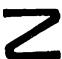
\includegraphics[keepaspectratio]{images/part002_676c5d74.jpg}}

Note that if the filtration on E is derived from that on A (Example 2), so is the quotient filtration on E/F, but not in general the filtration induced on F (Exercise 1; see however § 3, no. 2, Theorem 2).

If \(E'\) is another filtered A-module, the product filtration on \(E \times E'\) is compatible with its A-module structure. If the filtrations on E and \(E'\) are derived from that on A (Example 2), so is their product filtration.
